\documentclass[review]{elsarticle}

%\usepackage{natbib}
\usepackage{lineno,hyperref}
\usepackage{amsmath}
\modulolinenumbers[5]
\usepackage{graphicx}
\usepackage{caption}
\usepackage{subcaption}
\usepackage{tikz}

\usepackage[colorinlistoftodos]{todonotes}   % provides \todo for margin notes

\newcommand{\BoussClaw}{\textsc{BoussClaw} }
\newcommand{\BoussClawt}{\textsc{BoussClaw}}
\journal{Coastal Engineering}

%%%%%%%%%%%%%%%%%%%%%%%
%% Elsevier bibliography styles
%%%%%%%%%%%%%%%%%%%%%%%
%% To change the style, put a % in front of the second line of the current style and
%% remove the % from the second line of the style you would like to use.--00
%%%%%%%%%%%%%%%%%%%%%%%

%% Numbered
%\bibliographystyle{model1-num-names}

%% Numbered without titles--
%\bibliographystyle{model1a-num-names}

%% Harvard
%\bibliographystyle{model2-names.bst}\biboptions{authoryear}

%% Vancouver numbered
%\usepackage{numcompress}\bibliographystyle{model3-num-names}

%% Vancouver name/year
%\usepackage{numcompress}\bibliographystyle{model4-names}\biboptions{authoryear}

%% APA style
%\bibliographystyle{model5-names}\biboptions{authoryear}

%% AMA style
%\usepackage{numcompress}\bibliographystyle{model6-num-names}

%% `Elsevier LaTeX' style
\bibliographystyle{elsarticle-num-names}\biboptions{authoryear}
%%%%%%%%%%%%%%%%%%%%%%%

\begin{document}

\begin{frontmatter}

\title{Dispersive modeling of breaking waves  on a slope}

%% Group authors per affiliation:
\author[1]{Jihwan Kim}
\author[1]{Geir K. Pedersen}
\author[1,2]{Finn L{\o}vholt}
\author[3]{Randall J. LeVeque}

\address[1]{University of Oslo, Department of Mathematics, 
Oslo, Norway}
\address[2]{Norwegian Geotechnical Institute,
Oslo, Norway}
\address[3]{University of Washington, Department of Applied Mathematics, Seattle, USA}

\begin{abstract}

The nonlinear shallow water model is widely used
in the study of tsunami propagations,
but an increasing number of studies 
are dedicated to the dispersion dynamics of tsunamis.
If the wave dispersion becomes important,
Boussinesq-type models are often used. 
In this work, a general purpose Boussinesq solver, 
\BoussClawt, is introduced
for modeling fully non-linear dispersive tsunami propagation, 
taking into account inundation. 
In the \BoussClaw model,
Boussinesq equations from the literature, 
based on the depth-averaged velocity 
and with enhanced dispersion properties, 
are implemented using a hybrid of the finite volume
and finite difference methods.
In order to validate \BoussClawt, 
numerical results are compared 
to the analytical solutions and laboratory experiments. 
Furthermore, the  wave steepening and breaking motion
is carefully scrutinized, 
and we demonstrate that the point of wave breaking
may be wrongly identified  in many of the commonly used Boussinesq models. 

\end{abstract}

\begin{keyword}
Breaking wave, Boussinesq equation, finite volume method
\end{keyword}

\end{frontmatter}

\linenumbers

\section{Introduction}

Tsunamis are often considered as long waves compared to the water depth, and 
long-wave models are consequently widely used in the study of their propagation and inundation.
Through the use of numerical shock capturing techniques for modeling
the nearshore bore formation of the tsunami, {\em nonlinear shallow water} (NLSW) models
did become the standard model for modeling tsunami propagation and run-up, see e.g. 
\citep{titov1995modeling,Imamura1996b,Harig2008,BergerGeorgeLeVequeMandli11}.

The  NLSW models do not incorporate frequency dispersion, which may be included by ascending in the hierarchy of long wave expansion to the Boussinesq type 
equations. Numerical models based on Boussinesq type equations have been used
for idealized studies of wave processes since 1966 \citep{Peregrine:1966} and 
additionally to simpler problems in coastal engineering in the following decades \citep{Brocchini:2013}. 
However, the accumulated effect of the frequency dispersion for the wave propagation over the open sea is 
a function of propagation time and the shape of the disturbance \citep{Glimsdal2013},
and may become important for some tsunamis, in particular for landslide sources \citep{Lovholt2015}. 
Dispersion may further be of importance, in combination with non-linear effects,
for the evolution of undular bores for tsunamis \citep{Glimsdal2013,Grue:2008,Lovholt:2008b,Behrens2015}.
In the last decades we have seen a development on long wave expansions and their numerical formulations. 
In the 1990s the modeling with  Boussinesq type equations were vitalized by 
new formulations, in particular those of  \cite{madsen1992new} and \cite{nwogu1993alternative} which  displayed improved dispersion properties in comparison to the standard formulation of \cite{peregrine1967long}.
Later still more extensions and improvements have followed as described in the reviews \cite{Madsen:2003a}, \cite{Brocchini:2013} and \cite{Kirby:2016}.

 Boussinesq-type equations differ in mathematical structure from the NLSW equations and do not
inherit characteristics in the same simple form. Hence, other stratergies have been attempted for inclusion of wave breaking and  
post-breaking motion in Boussinesq models. 
\citet{schaffer1993boussinesq} employed the concept of the {\em surface roller},
first proposed by \citet{Svendsen:1984}, 
which is volume of water passively riding at
the bore front.
 Another way of incorporating the breaking that was suggested by \cite{Kennedy2000} who included diffusive terms
in the momentum equation which was activated and deactivated as a steepness measure crosses thresholds. The original steepness measure was the temporal rate of surface elevation corresponding to a very steep solitary wave.
Later, \citet{lynett2006nearshore} investigated a variety of steepness measures and
then identified that the surface steepness provides 
the least sensitive breaking threshold. 
 \citet{Lovholt:2013a} similarly employed a diffusive model including transport terms, but pointed out that breaking wave Boussinesq models were prone to instabilities. 
 \citet{tissier2012new} suggested
a breaking decision model based on the surface roller, the maximal front angle and the Froude number.
An alternative non-linear diffusive ad-hoc breaking term was suggested \citet{matsuyama2007study},
based on their large scale experiments of the wave propagation of undular bores on various slope angles. 
%They studied the wave breaking criteria and suggested 
%\begin{align*}
%\frac{u_s}{c} = \frac{\eta}{H} - \frac{h}{3H}
%\left(
%H\frac{\partial^2 \eta}{\partial x^2} - 2 \left(\frac{\partial \eta}{\partial x} \right)^2
%\right),
%\end{align*}
%as a wave breaking criterion.

However, there is a natural desire to exploit the efficient and well established shock capturing framework for NLSW models also in a dispersive context.
Hence, recently developed of  Boussinesq models are often based on hybrid numerical techniques
such as use of approximate Riemann solvers combined with TVD limiters for the conserved variables, and finite differences
for additional higher order terms \citep{Erduran2005,Kim2009,Shiach:2009,Roeber:2010,Dutykh:2011,shi2012high}. Among other models, this have led to the popular
\textsc{Funwave-TVD} and \textsc{Coulwave-TVD} applications. For instance in \citet{shi2012high}, Boussinesq terms are 
switched off the near-shore region where large amplitude-to-depth-ratios occur,
implying that only NLSW terms remain in the shallowest region.
This allows for a relatively robust treatment of the modeling of the post breaking phase. To this end,
the $A/h = 0.8$ threshold suggested by \citep{shi2012high} 
based on the Froude similarity analysis by \citet{tonelli2009hybrid}, have in many ways become the standard for incorporating
breaking in a feasible and practical way.

In this paper, we present a new hybrid Boussinesq type model \BoussClawt, 
of similiar mould as \textsc{Funwave-TVD} and \textsc{Coulwave-TVD}. The emphasis is twofold.
First, to present a careful validation of the model, both towards  
laboratory experiments and more general reference models. Second, we use the new model
in comparison with a full potential reference model to explore how accurate the Boussinesq models 
can represent the wave evolution until the point of breaking. In the present example,
we are finally able to demonstrate that Boussinesq models may be employed
to accurately model the near shore tsunami propagation beyond the standard $A/h = 0.8$ threshold depth.
Conversely, we find that the use of the standard $A/h = 0.8$ threshold depth 
invokes a too early formation of a breaking bore. This points out that  
that the breaking criteria employed so far lacks generality.
%While these criteria may be attractive due to robustness, 
%they may be lacking not only for modeling the breaking phase, but %in certain situation also the pre-breaking phase.
%\marginpar{\footnotesize Move to last part of this paragraph to conclusions (or omit this)?}

This paper is organized as follows: In Section \ref{sec:model}, the base model
for the wave equations is given and the numerical scheme is outlined, including a von Neuman stability analysis. 
Sections \ref{sec:num_nonbreaking} compares results from the \BoussClaw with
the analytic solutions and laboratory experiments. 
Section \ref{sec:wave_break} discusses the wave steepening and using a Boundary Integral Method (BIM) for 
solving the full potential equations. 
In Section \ref{sec:num_breaking}, 
we compare these results of pre-breaking
evolution with Boussinesq type models.

\section{Model Description}
\label{sec:model}

Boussinesq-type equations include non-hydrotstic pressure in an approximate way
treat short waves more accurately
than the shallow water equations. 
The Boussinesq-type wave models have been derived 
on the assumption that 
$\mathcal{O}(\epsilon)$ and $\mathcal{O}(\mu)$ terms
are small, where $\epsilon$ and $\mu$ 
denote the ratio of wave amplitude to depth
and the ratio of depth to wavelength respectively. 
Various models have been suggested,
and the papers of \citet{peregrine1967long},
\citet{madsen1992new}, \citet{nwogu1993alternative},
\citet{lynett2002modeling},
and \citet{wei1995time}
are representative examples. 

In this work, a new numerical model, 
called \BoussClawt, is introduced. 
It is an extension of \textsc{Geoclaw} \citep{clawpack},
and solves 
the Boussinesq-type equations derived by
\citet{schaffer1993boussinesq}.
The \BoussClaw model
is a hybrid of the finite volume and finite difference solvers
with the fractional step technique.
The \textsc{Geoclaw} software is 
a part of \textsc{Clawpack} \citep{clawpack}
developed mainly by
\citet{leveque1997wave}, \citet{george2008augmented}
and \citet{BergerGeorgeLeVequeMandli11},
which is designed to solve the nonlinear shallow water equations.
%with properties such as high-resolution, total variation diminishing (TVD) and adaptive mesh refinements (AMR).
% The wave propagation algorithms by LeVeque (1997) \cite{leveque1997wave} is implemented, and the steady state is preserved. 

\subsection{\BoussClaw - a new long wave model for tsunami propagation and run-up}

\subsubsection{Boussinesq-type equations}

\citet{schaffer1993boussinesq} derived 
Boussinesq-type equations
with an addition of a Pad{\'e} approximation 
of the linear dispersion relation.
The equations read 
\begin{flalign}
& H_t + (Hu)_x  = 0, \label{eq:madsen_cons_mass} & \\ 
& (1-D)\big\lbrack(Hu)_t\big\rbrack + \left( Hu^2 + \frac{g}{2}H^2 \right)_x - gHh_x -Bgh^2\left(h\eta_x\right)_{xx} =0, \label{eq:madsen_momx} &
\end{flalign}
where the operator $D$ is defined as
\begin{flalign}
 D (w) &= \left(B+\frac{1}{2} \right)h^2 w_{xx} -\frac{1}{6} h^3 \left(\frac{w}{h}\right)_{xx}, & \label{eq:madsen_new_op}
\end{flalign}
for any $w(x,t)$.
In the above equations $H(x,t)$ and $u(x,t)$ are the total flow depth and the depth averaged velocity of the water, respectively, 
$h(x)$ is the still water depth, $\eta(x,t)$ is the surface elevation,
and thus $H(x,t)=h(x)+\eta(x,t)$. 
Moreover, $g$ is the acceleration of gravity, 
and $B$ is a dispersion parameter. 
\citet{madsen1992new} 
have chosen the parameter $B=1/15$ 
from a Pad{\'e}
expansion of the linear dispersion analysis.
When $B=0$, this set of the Boussinesq-type equations
approximately reduces to that of \citet{peregrine1967long}
as the linear dispersion relations are identical. 
However, unlike Peregrine's momentum equation 
the hydrostatic parts of (\ref{eq:madsen_momx}) 
are written in a conservative form. Moreover, some nonlinearity is introduced
in the dispersion term for convenience. 
Even though (\ref{eq:madsen_cons_mass}), 
(\ref{eq:madsen_momx}) and (\ref{eq:madsen_new_op}) do not constitute a fully nonlinear set of Boussinesq equations, 
they do describe shoaling of solitary waves markedly
better than, for instance, the Peregrine equations, as will be demonstrated in 
section  \ref{sec:num_breaking}.


The \BoussClaw model
solves the Boussinesq-type equations (\ref{eq:madsen_cons_mass}) and (\ref{eq:madsen_momx}) numerically
with a hybrid combination of the finite volume and finite difference methods that will be explained in a moment. 
There have been several studies of this type of hybrid schemes.
For example, see \citet{tissier2011serre}, \citet{shi2012high} and \citet{dutykh2013finite}.


To facilitate a fractional step method, as outlined below, we move the hydrostatic terms of (\ref{eq:madsen_momx}) inside the $(1-D)$ 
operator, while balancing with extra terms in the $\Psi$, to obtain
\begin{flalign}
& (1-D)\big\lbrack (Hu)_t + \left(Hu^2 + \frac{g}{2}H^2 \right)_x - gHh_x\big\rbrack = -\Psi(x,t), & \label{eq:hybrid_src}
\end{flalign}
where
\begin{flalign}
\Psi(x,t)= & \left(B+\frac{1}{2} \right) h^2 \left( (Hu^2)_{x} + g H \eta_x \right)_{xx} \nonumber\\
& -\frac{1}{6}h^3 \left( \frac{ (Hu^2)_x +gH\eta_x }{h} \right)_{xx}
-Bgh^2\left(h\eta_x\right)_{xx}. &
\label{eq:madsen_new_disp_x}
\end{flalign}

\subsubsection{Numerical scheme}
\label{sec:Num_scheme}
The equations (\ref{eq:madsen_cons_mass}) and (\ref{eq:hybrid_src}) are 
written in a form that conserves momentum to leading order in $\mu$, but with the $\Psi$
term as a pseudo source.
Such equations may be solved  
by a {\em fractional step method} as described in  
\citet{leveque2002finite},
for instance. 
First, it is observed that (\ref{eq:hybrid_src}) may be formally
rewritten as 
\begin{flalign}
& (Hu)_t =- \left\lbrace\left(Hu^2 + \frac{g}{2}H^2 \right)_x - gHh_x\right\rbrace -(1-D)^{-1}\Psi(x,t), & \label{eq:hybrid_inv}
\end{flalign}
At the first stage of the hybrid scheme, we integrate $Hu$ over a time step
taking into account all hydrostatic terms, namely 
those within the braces on the right hand side, and omitting the source terms involving $\Psi$. 
When this is combined with the continuity equation
(\ref{eq:madsen_cons_mass}) this simply corresponds to advancing 
the shallow water equations one time step forward. 
To this end we employ \textsc{Geoclaw},
a high-order accurate finite volume solver 
for the shallow water equations with adaptive mesh refinements.

%\marginpar{\small add a descriptio of the NLSW procedure}

In the second stage, we retain the new $H$ value, but integrate $Hu$ (essentially being the momentum density) further 
from the first stage by solving
\begin{flalign}
& \left(1-D \right)\big\lbrack (Hu)_t\big\rbrack = -\Psi . & \label{eq:hybrid_mom_fdm}
\end{flalign}
Since the differential operator $D$ contains spatial derivatives,
a systems of difference equations must then be solved. 

The spatial and time discretization should be carefully chosen 
for the stability of the second stage. 
In our numerical scheme, the second order centered scheme
is used for the spatial discretization, 
and a four stage Runge-Kutta method is used for the time integration.
The von Neumann stability analysis of this numerical scheme 
is outlined in \ref{append:stab}.

Suppose the spatial domain is divided into $n$ grid cells with 
the spatial grid size $\Delta x$.
Arrays of nodal values for flow depth and $Hu$, respectively, are
defined as
\begin{flalign*}
\textbf{H} & =
(H_1,H_2, \dots , H_n)^T, & \\
\textbf{M} & =
(H_1u_1,H_2u_2, \dots , H_nu_n)^T. &
\end{flalign*}

With time increment $\Delta t$ the fourth order Runge-Kutta scheme
can be written as follows,
\begin{flalign}
\textbf{M}^1 = \textbf{M}, \quad 
\textbf{M}^2 = \textbf{M} + \frac{\Delta t}{2}\textbf{S}^1, \quad
\textbf{M}^3 = \textbf{M} + \frac{\Delta t}{2}\textbf{S}^2, \quad
\textbf{M}^4 = \textbf{M} + \Delta t \textbf{S}^3,
\label{eq:rk4_S}
\end{flalign}
where $\textbf{M}^k$ are intermediate value arrays
%\marginpar{How are values for $H$ obtained in the steps; linear interpolation ?} 
and $\textbf{S}^k$ are
correpondingly arrays for the time derivatives of $Hu$, obtained by
solving 
\begin{flalign}
(I-\bar{D})\textbf{S}^k & 
= -\bar{\Psi}(\textbf{H},\textbf{M}^k), \quad \textrm{for~} k=1,\dots,4. &
\label{eq:rk4_1}
\end{flalign}
Here $\bar{\Psi}$ and $\bar{D}$ represent centered spatial discretizations for the term $\Psi$ and the operator $D$, respectively. These
are given explitly below.
Finally the value of $\textbf{M}$ at the new time level is
obtained by
\begin{flalign}
\textbf{M}^+ & = \textbf{M} + \frac{\Delta t}{6} \left[
\textbf{S}^1+2\textbf{S}^2+2\textbf{S}^3+\textbf{S}^4
\right]. 
\label{eq:rk4_assemble}
\end{flalign}

In (\ref{eq:rk4_1}), 
$\bar{D}$ is a tri-diagonal $n\times n$ matrix with elements 
\begin{flalign*}
 \bar{D}_{i,i-1} = & \frac{1}{\Delta x^2} \left[
 \left(B + \frac{1}{2} \right) h_i^2 
-\frac{1}{6} \frac{h_i^3}{h_{i-1}} \right],  & \\
 \bar{D}_{i,i} = & \frac{1}{\Delta x^2}
 \left(-2B - \frac{2}{3} \right) h_i^2 ,  & \\
 \bar{D}_{i,i+1} = & \frac{1}{\Delta x^2} \left[
 \left(B + \frac{1}{2} \right) h_i^2 
-\frac{1}{6} \frac{h_i^3}{h_{i+1}} \right].  & 
\end{flalign*}
Correspondingly, the $i$-th element of $\bar{\Psi(\textbf{H},\textbf{q})}$ is 
\begin{flalign*}
\bar{\Psi}_i 
&=  \left(B+\frac{1}{2} \right) \frac{h_i^2}{2\Delta x^3} 
\Bigg[
\left(\frac{M_{i+2}^2}{H_{i+2}} -2\frac{M_{i+1}^2}{H_{i+1}} 
+2\frac{M_{i-1}^2}{H_{i-1}}-\frac{M_{i-2}^2}{H_{i-2}} \right) \\
& +g\left(H_{i+1}\left(\eta_{i+2}-\eta_{i}\right)
-2H_{i}\left(\eta_{i+1}-\eta_{i-1}\right) 
+H_{i-1}\left(\eta_{i}-\eta_{i-2}\right) \right)\Bigg]  \\
& -\frac{1}{6}\frac{h_i^3}{2\Delta x^3} \Bigg[
 \frac{M_{i+2}^2/H_{i+2}-M_i^2/H_i}{H_{i+1}}
 -2\frac{M_{i+1}^2/H_{i+1}-M_{i-1}^2/H_{i-1}}{h_{i}} \\
& +\frac{M_{i}^2/H_{i}-M_{i-2}^2/H_{i-2}}{H_{i-1}}
 \\
 &+ g \left( \frac{H_{i+1}(\eta_{i+2}-\eta_{i})}{H_{i+1}} 
 -2 \frac{H_{i}(\eta_{i+1}-\eta_{i-1})}{h_{i}} 
 + \frac{H_{i-1}(\eta_{i}-\eta_{i-2})}{H_{i-1}} 
 \right) \Bigg] \\
& -\frac{Bgh_i^2}{2\Delta x^3}
\left( H_{i+1}\left(\eta_{i+2}-\eta_{i} \right)
-2H_{i}\left(\eta_{i+1}-\eta_{i-1} \right)
+H_{i-1}\left(\eta_{i}-\eta_{i-2} \right) \right), &
\end{flalign*}
for $i=1,2,\dots,n$.
\subsubsection{Additional numerical features}
\label{sec_add_num}
Following \cite{shi2012high} we may catch wave breaking in a heuristic fashion 
through  invokation of a threshold $\epsilon_B:=\eta/h=0.8$ in \BoussClaw.
When the threshold is reached, the wave breaking is supposed to be initiated, 
and the dispersive terms are suppressed. 
At the breaking, the set of equations is locally 
switched to the shallow water equations for the corresponding leading wave, %packet\todo{G: wave packet is too loose. Must specify.},
and the trailing waves are solved with the Boussinesq equations
if the thresholds are not reached. 


When a wave reaches the coastline, 
the coastline changes in time
as the wave runs up the slope and recedes eventually. 
For the numerical simulations, 
it has been a challenge to compute the inundation correctly.
At the coastline above the sea level, \BoussClaw
switches to the NLSW solver of the \textsc{Geoclaw} software,
%\todo{RJL: I modified this sentence, is this correct?}
which can handle 
wet and dry states with the depth positivity property.
Details can be found in \cite{george2008augmented}. 

Friction terms are important for inundation on gentle slopes. 
For example, the Figure \ref{fig:BoussClaw_runup}
shows that the run-up height is much reduced by the friction terms.
\BoussClaw uses the Manning-type frictions as follows,
\begin{flalign*}
f_D = -\frac{g C_d^2 u |u|}{H^{5/3}},
\end{flalign*}
where $C_d$ is a Manning drag coefficient.
Another parameter $d^*$ needs to be chosen
so that the water depth is set to $H=0$
if the water depth is smaller than this threshold, $H<d^*$.
\cite{antuono2012role} derived an approximate solution
of the shoreline for the shallow water equations 
with the Chezy friction,
and studied the effect of the frictional coefficient and 
the water depth tolerance.
In this work, the parameter $d^*$ is set to $10^{-4}$. 


\subsection{Models for comparison}
The performance of the Boussinesq model presented here is 
assessed by comparison with numerical results from a full potential
flow model which is described in \citet{Lovholt:2013a} and references therein. The model is based on a boundary 
integral technique and is run  with fully nonlinear solitary
wave solutions as initial conditions. During shoaling and breaking this
model can describe the evolution of a plunger, but breaks down
when the plunger reaches the free surface. Hence, the potential flow 
results are used to determine the point of breaking due to shoaling 
and to
evaluate the evolution of  amplitude and wave 
shape of the current model until this point.   
Below we refer to the full potential model as the BIM (Boundary
 Integral Method) model.

Comparison with a pre-existing, fully nonlinear Boussinesq model is
facilitated by the application of a Lagrangian model, described
in \citet{Lovholt:2013a}. Apart from the use of
Lagrangian coordinates the equations employed in this model are
 similar to (\ref{eq:madsen_cons_mass}) and (\ref{eq:madsen_momx}).
They differ only concerning the nonlinearities in the
dispersion terms and that  the dispersion optimization terms are added in a fully nonlinear fashion.
Presently, the Lagrangian model has no established bore capturing 
facility and is hence valid only to the point of breaking.
Results from this model will be referred to as 'Serre', even though
the dispersion enhancement is invoked. 
 
Results for the Peregrine-type Boussinesq equations are obtained by the
GloBouss model. This is a dispersive tsunami propagation model which
is based on Peregrine-type equations and discretization on a staggered grid. Further details are found in 
\citet{Lovholt:2008b}.

For comparison also the version 2.1 of the  \textsc{Funwave-TVD} model
by \citet{shi2012high} is used. The
\textsc{Funwave-TVD} model shares important features with \BoussClawt, employing a hybrid 
of the finite volume and finite difference
scheme to solve the fully non-linear higher order dispersive Boussinesq model numerically.
While we refer to \citet{shi2012high} for details, we briefly note that \textsc{Funwave-TVD} is based the fully nonlinear 
Boussinesq equations of \citet{Chen06}. The numerical spatial representation in \textsc{Funwave-TVD} is MUSCL TVD scheme 
to discretize for the flux and first order terms, 
whereas a central finite difference
scheme \citet{Wei95} is utilized for the higher order momentum terms. A Runge-Kutta scheme is employed for the time stepping.

\section{Numerical Tests}
\label{sec:num_nonbreaking}

\subsection{Solitary wave propagation}

In order to validate the numerical approach 
a solitary wave propagation is tested on a constant water depth.
For the initial conditions, 
the analytic solitary wave solution 
of the Serre's equations is used
since analytic solutions are unknown 
for
the set (\ref{eq:madsen_cons_mass}) and 
(\ref{eq:madsen_momx}).
Solitary wave solutions to Serre's equations are given as
\begin{flalign}
\label{eq:anal_serre}
\begin{split}
& \eta(x,t) = A\, \textrm{sech}^2 \left( \kappa (x-ct)\right),  \\
& u(x,t) = c \frac{\eta(x,t)}{h},
\end{split} &
\end{flalign}
where
\begin{flalign}
\begin{split}
& \kappa = \frac{\sqrt{3h}}{2A\sqrt{A+h}}, \quad \textrm{and}
 \quad c = \sqrt{g\left( A + h \right)}.
\end{split} &
\end{flalign}
In this expression, $A$ and $h$ are constants
which represent the wave amplitude and the undisturbed water depth
respectively.

In Figure \ref{fig:soliton_ts}, 
snapshots from the \BoussClaw simulation are shown 
at $t=0,4,8$ and $12$ with $\Delta x = 0.1$. 
For the initial conditions, the solution (\ref{eq:anal_serre})
is used with $A=0.2$, $h=1$ and $g=9.81$.
The computational results are in good agreement 
with the analytic solutions concerning height, shape and propagation speed. 
The amplitudes decreases very gently as the wave propagates. 
%The discreapancy may be  partially due to the numerical errors
%and partly to the fact that 
%the analytic solution for Serre's equations satisfies
%the present Boussinesq-type equations only approximately.

\begin{figure}[!htb]
\centering
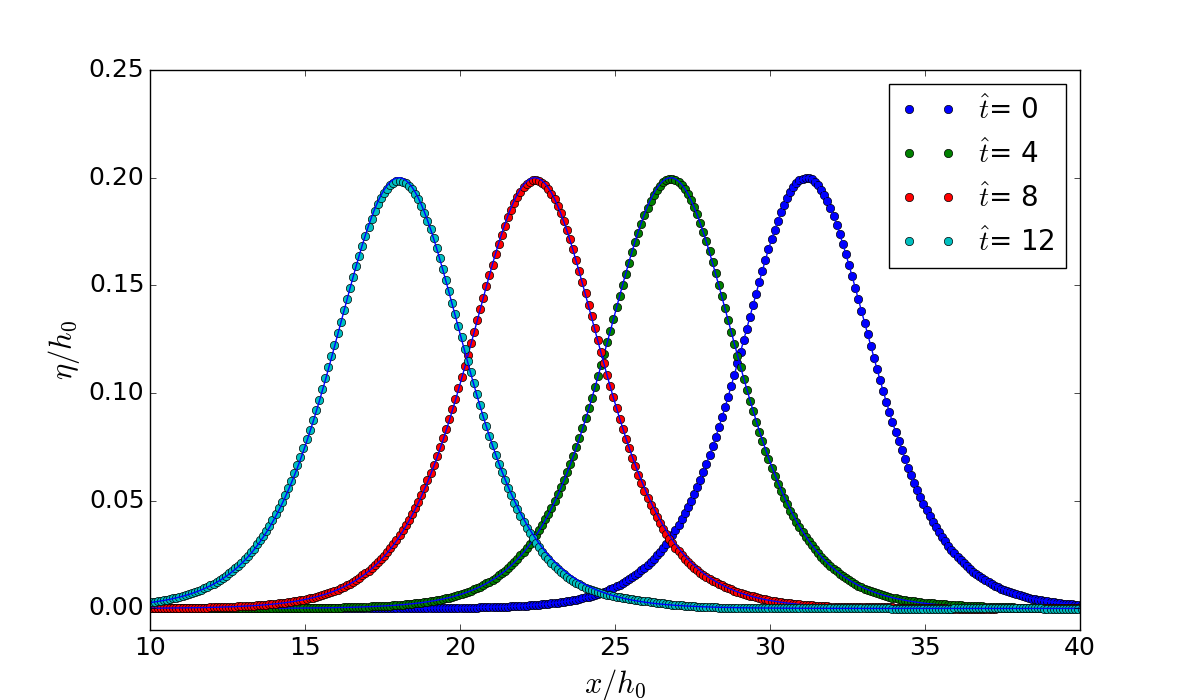
\includegraphics[width=.8\textwidth]{_fig/soliton_ts.png}
\caption{Snapshot of the analytic and computed solitary wave 
at $t=0,4,8$ and $12$ with $A/h=0.2$. 
The wave propagates from right to left,
and the analytic solutions are black solid lines.}
\label{fig:soliton_ts}
\end{figure}

The verically integrated wave energy densities for the shallow water equations 
and the Boussinesq equations are $e_0$ and $e_0+e_1$, respectively, where
\begin{flalign}
& e_0 = \frac{1}{2}\left( g\eta^2 + H\bar{u}^2 \right), \label{eq:energy_e0} \\
& e_1 = \frac{1}{6}H^3\bar{u}_x^2
+ \frac{1}{2}H^2h_x\bar{u}\bar{u}_x + \frac{1}{2}Hh_x^2\bar{u}^2.
\label{eq:energy_e1}
\end{flalign}
Details are given in \citet{madsen1997surf} 
and \ref{append:energy}. When the densities are integrated over the whole 
horizontal domain we obtain the corresponding total energies (per width), 
denoted as $E_0$ and $E_1$.

%The wave energy is conserved 
%as long as the wave is smooth and do not break,
%and the energy decreases as the wave breaks.
%The energy can be divided into the potential energy and kinetic energy, and the potential energy of $E_0+E_1$ is $\frac{1}{2} g\eta^2$.

\begin{figure}[!htb]
    \centering
    \begin{subfigure}[b]{0.45\textwidth}
        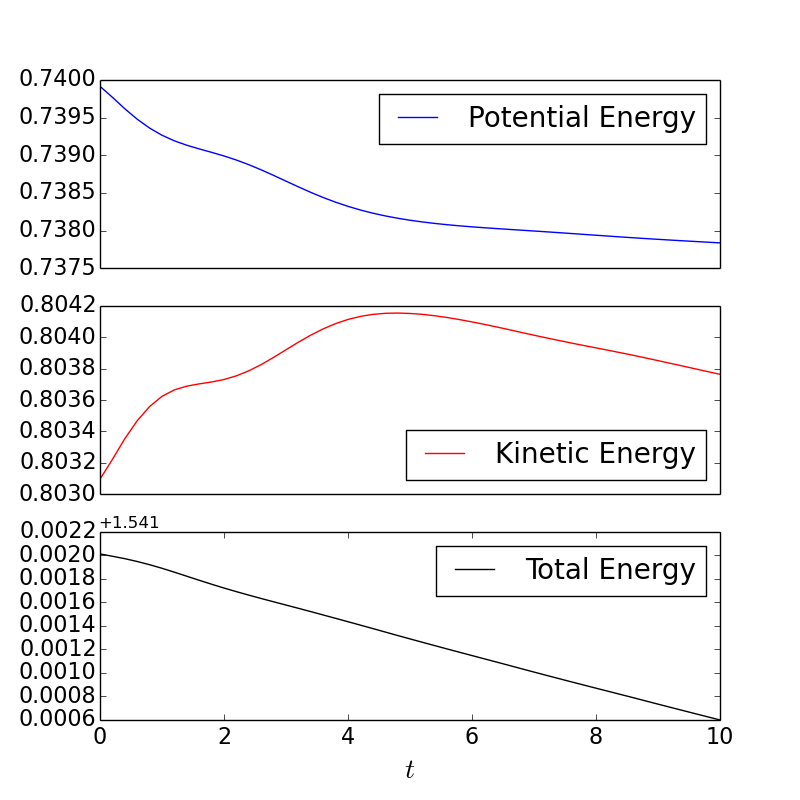
\includegraphics[width=\textwidth]{_fig/soliton_energy.png}
        \caption{Energy}
        \label{fig:soliton_energy}
    \end{subfigure}
    \begin{subfigure}[b]{0.45\textwidth}
        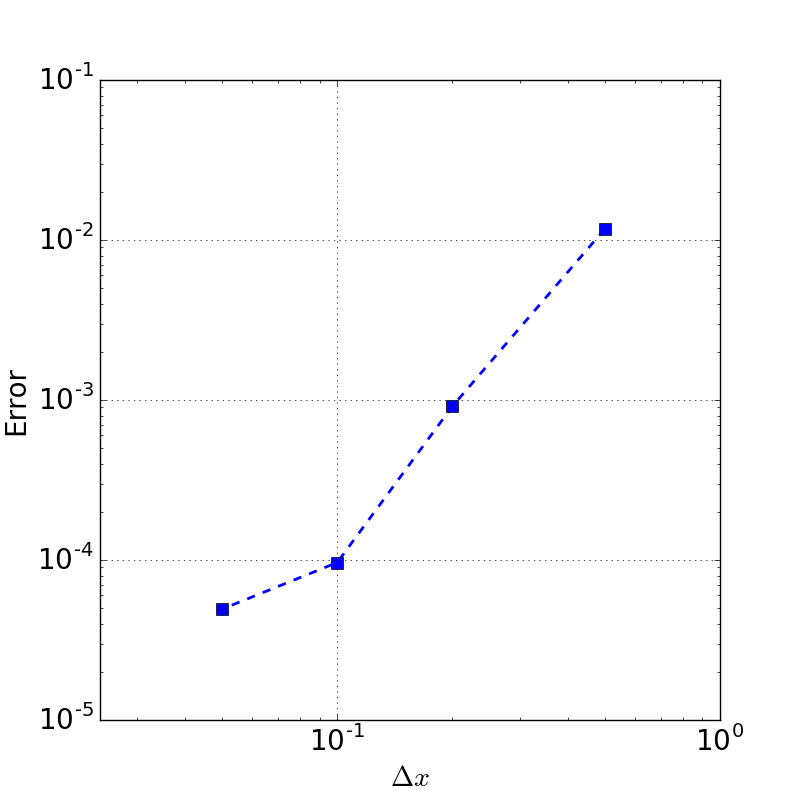
\includegraphics[width=\textwidth]{_fig/soliton_energy_dx.png}
        \caption{Relative error of energy}
        \label{fig:soliton_energy_dx}
    \end{subfigure}
    \caption{The energy of a solitary wave
    with $\Delta x = 0.2$ (left), 
    and log-log plot of relative error 
    at $t=10$ for $\Delta x = 0.05, 0.1, 0.2$ and $0.5$ (right).}
    \label{fig:soliton_error_energy}
\end{figure}

In Figure \ref{fig:soliton_energy}, the energy of the solitary
wave is shown with $A/h=0.2$ and $\Delta x = 0.2$.
There are fluctuations both in the potential and kinetic energy that is evident when we zoom in,
and the total energy decreases 
showing that the numerical procedure has dissipation.
In Figure \ref{fig:soliton_energy_dx},
the relative error of the energy at $t=10$,
\begin{flalign*}
Error = \frac{\left| E_{t=0}-E_{t=10} \right|}{\left|E_{t=0}\right|}, &
\end{flalign*}
is shown for different $\Delta x$.
For a solitary wave on a constant depth,
the energy dissipation decreases with the grid increments.

\subsection{Waves on a composite slope}

A physical model was constructed at the Coastal Hydraulic Laboratory of the U.S. Army Corps of Engineers
in order to address beach erosion and severe flooding problems \citet{chl_bp5}. 
The model beach consists of three piecewise linear slopes of 1:53, 1:150, and 1:13 with a vertical wall at the shoreline as shown in Figure \ref{fig:bp5_water_tank}.
In the laboratory, the wavemaker was located at 23.23 m.
The gauge data from three cases are provided 
where the ratio $A/h$ is equal to $0.038$, $0.259$ and $0.681$
with $h=21.8$ cm.

\begin{figure}[!htb]
\centering
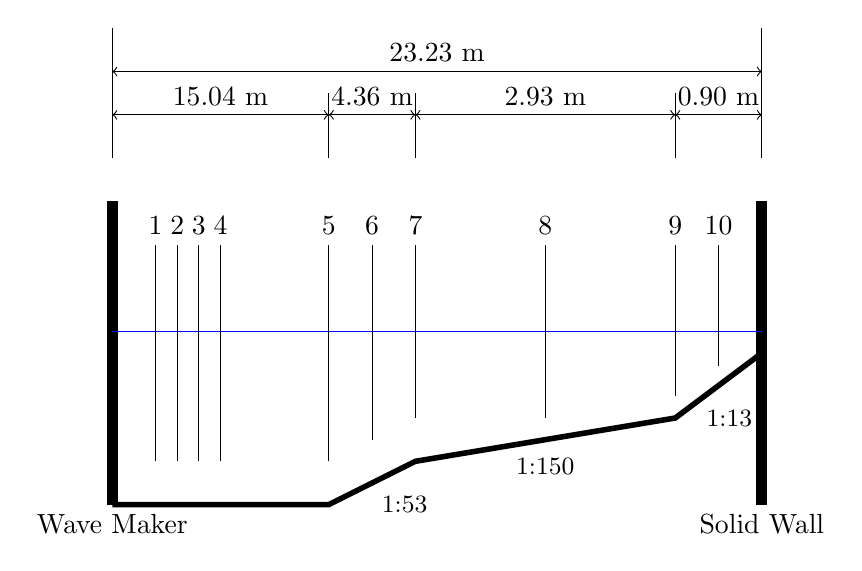
\begin{tikzpicture}[scale=.55]
 \draw[line width=4pt] (0,-4) -- (0,3);
 \draw[line width=2pt] (0,-4) -- (5,-4) -- (7,-3) --(13,-2) -- (15,-0.5);
 \draw[line width=4pt] (15,-4)--(15,3);
 \node[below] at (0,-4) {Wave Maker};
 \node[below] at (15,-4) {Solid Wall};
 \draw[blue] (0,0) -- (15,0);
 \draw (1,-3) -- (1,2) node[above]{1};
 \draw (1.5,-3) -- (1.5,2) node[above]{2};
 \draw (2,-3) -- (2,2) node[above]{3};
 \draw (2.5,-3) -- (2.5,2) node[above]{4};
 \draw (5,-3) -- (5,2) node[above]{5};
 \draw (6,-2.5) -- (6,2) node[above]{6};
 \draw (7,-2) -- (7,2) node[above]{7};
  \draw (10,-2) -- (10,2) node[above]{8};
 \draw (13,-1.5) -- (13,2) node[above]{9};
 \draw (14,-0.8) -- (14,2) node[above]{10};
 \node[right] at (6,-4) {\small 1:53};
 \node[below] at (10,-2.7) {\small 1:150};
 \node[right] at (13.5,-2) {\small 1:13};
 \draw (0,4) -- (0,7);
 \draw (15,4) -- (15,7);
 \draw[<->] (0,6) -- (15,6);
 \node[above] at (7.5,6) {23.23 m};
 \draw[<->] (0,5) -- (5,5);
 \node[above] at (2.5,5) {15.04 m};
 \node[above] at (6,5) {4.36 m};
 \draw[<->] (5,5) -- (7,5);
 \node[above] at (10,5) {2.93 m};
 \draw[<->] (7,5) -- (13,5);
 \draw[<->] (13,5) -- (15,5);
 \node[above] at (14,5) {0.90 m};
 \draw (5,4) -- (5,5.5);
 \draw (7,4) -- (7,5.5);
 \draw (13,4) -- (13,5.5);
  \end{tikzpicture}
  \caption{A sketch of the water tank}
  \label{fig:bp5_water_tank}
\end{figure}

The second case with $A/h=0.259$ has been 
compared with the numerical tests
which employed $400$ grid points. 
%And the switching scheme between the shallow water equations and the Boussinesq equations, is not applied.
To specify the incoming wave from the left boundary, 
the data at Gauge 4 were used for the wave height,
and the corresponding velocity (\ref{eq:anal_serre})
was applied.

In Figure \ref{fig:bp5b_gauges}, water surface elevations at gauges 5, 7 and 8 are shown. 
The simulated waves are in good agreement with the laboratory measurements. 
For the reflected waves, larger discrepancies are observed.
The increased discrepancy occurs because the full interaction between the wave and the wall
at the right boundary is less accurately captured.
Friction forces influence the wave evolution along the shallow region near the right wall,
but we have not included these in the present numerical simulation.
A better fit may possibly be obtained by incorporating friction, however,
tuning the friction models is not the scope of this work. 

\begin{figure}[!htb]
\centering
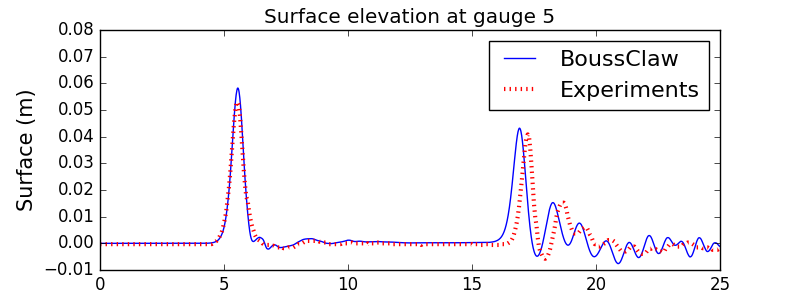
\includegraphics[width=.8\textwidth]{_fig/gauge0005fig300.png}\\
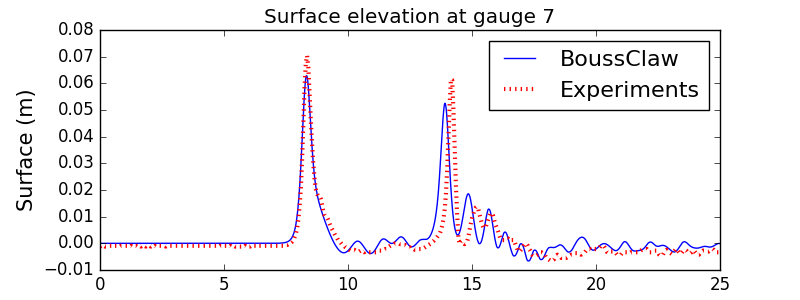
\includegraphics[width=.8\textwidth]{_fig/gauge0007fig300.png}\\
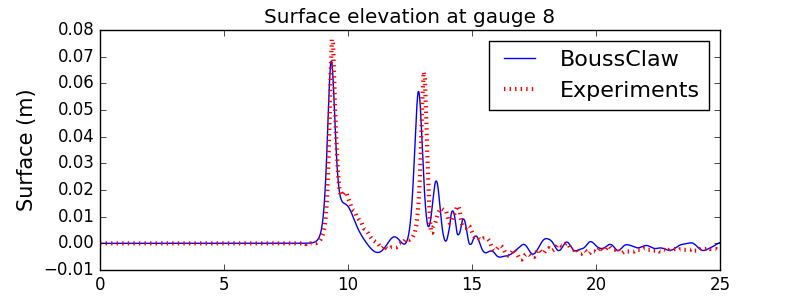
\includegraphics[width=.8\textwidth]{_fig/gauge0008fig300.png}
\caption{Water surface elevation at gauges 5,7 and 8 for $A/h=0.269$ case.}
\label{fig:bp5b_gauges}
\end{figure}

%\marginpar{\footnotesize Geir: A very shallow region may yield %important frictional effects? But, surely, the wave should  break %in the shallowest region?}
\subsection{Runup on a steep slope}
\label{sec:10degrunup}
On a $10^\circ$ slope an incident solitary wave of amplitude $A/h=0.3$ will not break until the end of the draw-down phase \cite{Grilli:1997}.
Still, this may be a challenging task for Boussinesq type models \citep{Lovholt:2013a}. Runup on a $10^\circ$ was investigated experimentally
by \citet{Pedersen:2013} who found a theoretical overshoot of roughly 20\% in the maximum runup height. This was alloted to the viscous boundary layer on the beach and capillary effects. Moreover, the measurements showed that the boundary layer flow during runup was mostly laminar, albeit indications of transition was observed in the upper part of the swash tongue close to flow reversal. Hence, it is not appropriate to employ a Manning friction term and we compare the models without any bed friction, while leaving the experiments out. 

\subsection{Comparsion with experiments on a breaking wave}
\label{sec:wave_break}

%Depth-averaged models are not capable of handling the wave breaking unless they are modified by incorporating the energy dissipation. In this work, a breaking solitary wave will be considered on a uniform slope. For laboratory experiments, see Synolakis \{synolakis1987runup}.

\citet{synolakis1987runup} performed a series of laboratory expseriments for the run-up of solitary waves
on uniform slopes. Here, we are interested in the  breaking cases. 
One such example in \citet{synolakis1987runup} is a solitary wave of amplitude $A/h=0.28$ 
approaching a slope of $1:19.85$. In Figure \ref{fig:init_setup}, the initial set-up for a test is shown. 
%, and the experiment results include various cases with the wave amplitudes and slope angles. Synolakis identified the breaking and non-breaking wave cases. 

\begin{figure}[!htb]
\centering
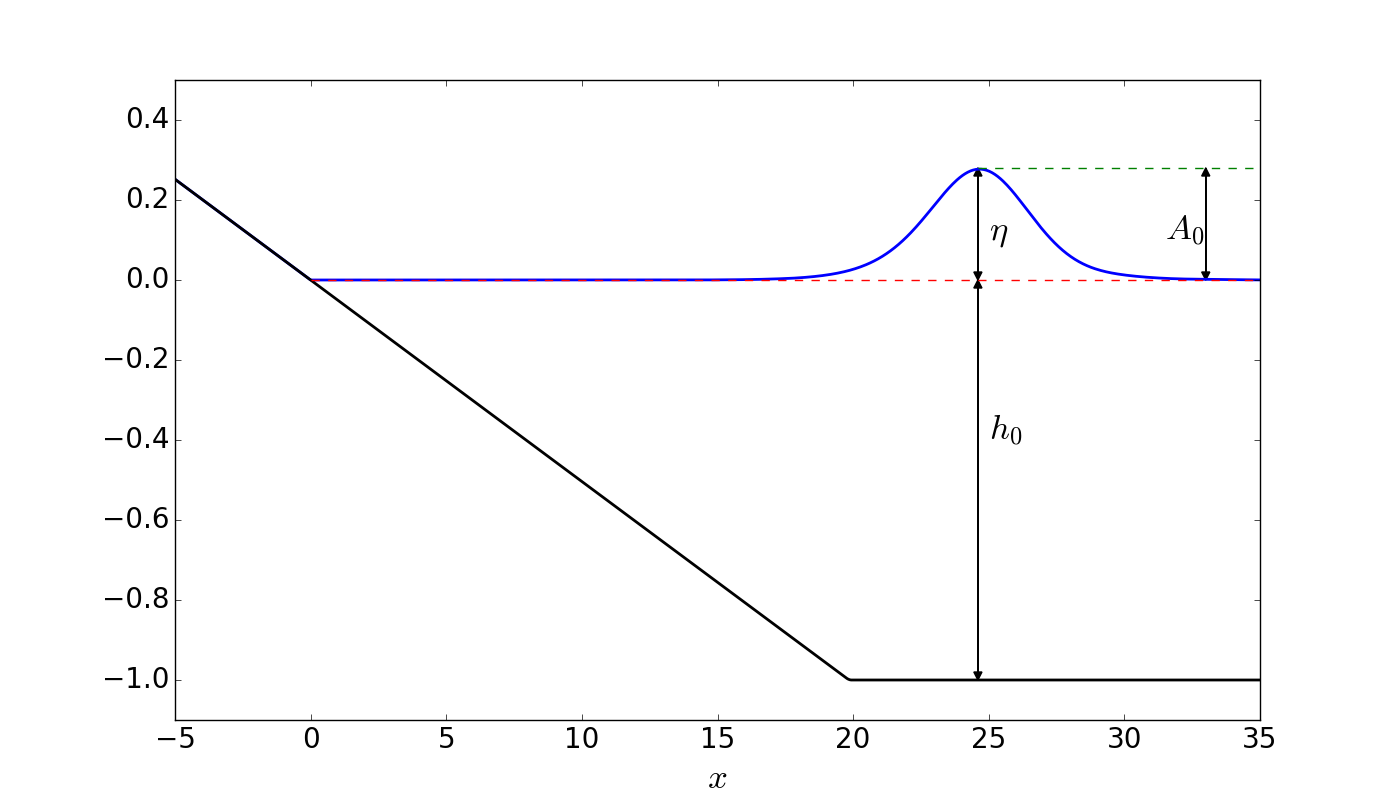
\includegraphics[width=.7\textwidth]{_fig/initial_setup.png}
\caption{Set-up of a numerical test for Synolakis' experiments.}
\label{fig:init_setup}
\end{figure}

The set-up of the wave tank in the simulations follows the laboratory experiments by \citet{synolakis1987runup}. 
The bathymetry of the wave tank is composed of a horizontal bottom and 
a uniform slope as shown in Figure \ref{fig:init_setup}. 
A solitary wave of amplitude $A/h=0.28$ is generated at the right end of
the tank and propagates leftwards
to the beach. 

We present the results using the non-dimensional time 
$t^*=t\sqrt{h/g}$ and non-dimensional space $x^*=x/h$. In the following, we drop the asterisks in 
the presentation of the results. 
In  \citet{synolakis1987runup}, $t=0$ was defined as when the wave crest was a non-dimenional distance, $L$, from the toe of the slope,
where
\begin{flalign*}
& L = \sqrt{\frac{4A}{3h}} \textrm{arccosh} \left( \frac{1}{0.05} \right). &
\end{flalign*}
However, at $t=0$, the solitary wave has an elevation of
5\% of it maximum at the toe of the beach, meaning that the slope has
started to interact with the solitary wave. To avoid any such interaction obscuring
our analysis, we instead place the initial solitary wave using equation (\ref{eq:anal_serre}) 
at $L + 5c$, where $c$ is the shallow water wave celerity.
In this way, the initial solitary wave has a negligible interaction with the slope when initialized. 
%Then $t=0$ is set as soon as the peak of wave is at $x=L$.

In Figure \ref{fig:lab_bim}, the laboratory measurements
are shown with the computational results from the \BoussClaw (in Boussinesq and NLSW mode) and the BIM models
for $A/h=0.28$ and a $1:19.85$ slope at $t=15$. 
The grid size $\Delta x$ is 0.05 in the following simulations
unless stated otherwise.
This is before the wave breaks and
both \BoussClaw and the BIM model are in good agreement with the experiments.
%\marginpar{\footnotesize Also include the BoussClaw results and NLSW in fig.~\ref{fig:lab_bim}}.

\begin{figure}[!htb]
\centering
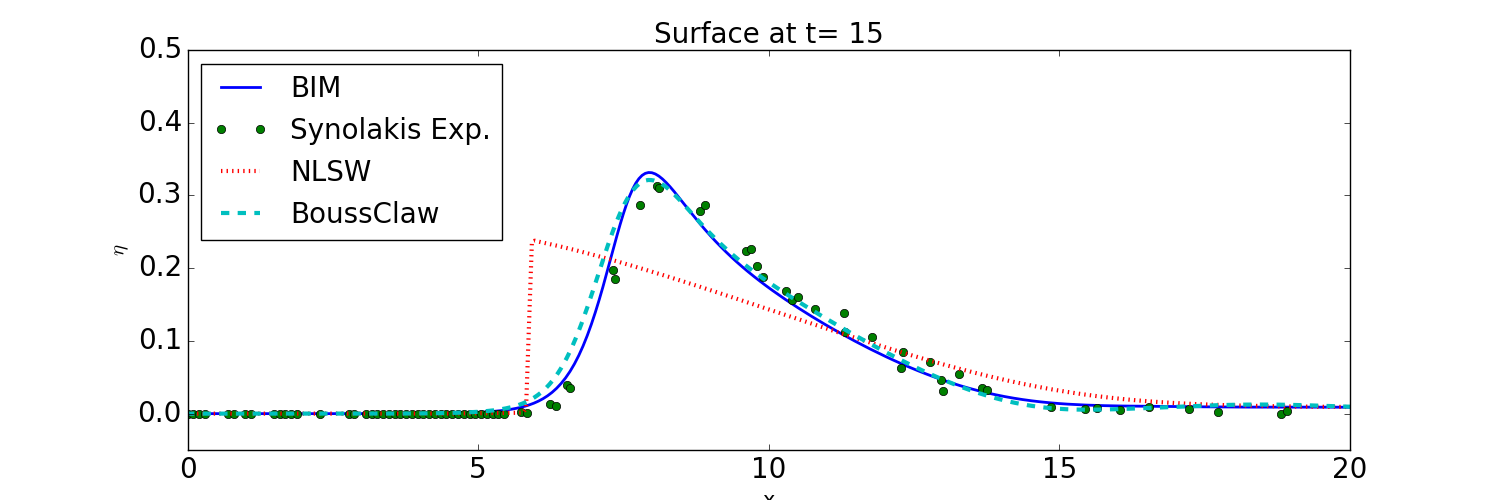
\includegraphics[width=\textwidth]{_fig/lab_bim_t15.png}
\caption{Comparison of the laboratory experiments, BIM, NLSW and BoussClaw at t=15 with $A/h=0.28$ 
on a slope of $1:19.85$.}
\label{fig:lab_bim}
\end{figure}

%\marginpar{\footnotesize What is the result of Titov and Synolakis?} 
%and the undisturbed depth is $h=0.206$ m. 
The ratio of amplitude to depth, $A/h$, 
is about $2.01$ at the break point.
The potential flow model cannot be run much beyond the
breaking points (until the attachment of the plunger only) and 
gives no information on the following bore propagation.
In figure \ref{fig:BoussClaw_runup} we have compared the \BoussClaw model, with and without 
a Manning friction, with the experimental data. The agreement is good and the introduction of bed-friction 
even seem to match the truncated swash tongue of the experiments well. However, this may be a coincidence. Even though
the  wave has broken and some irregular flow features are introduced thereby, we have no evidence of the flow state being
anywhere near turbulent, which is required for a quadratic bottom resistance to be appropriate. Capillary effects and 
experimental errors may also affect the comparison.
\begin{figure}[tbh!]
	\centering
	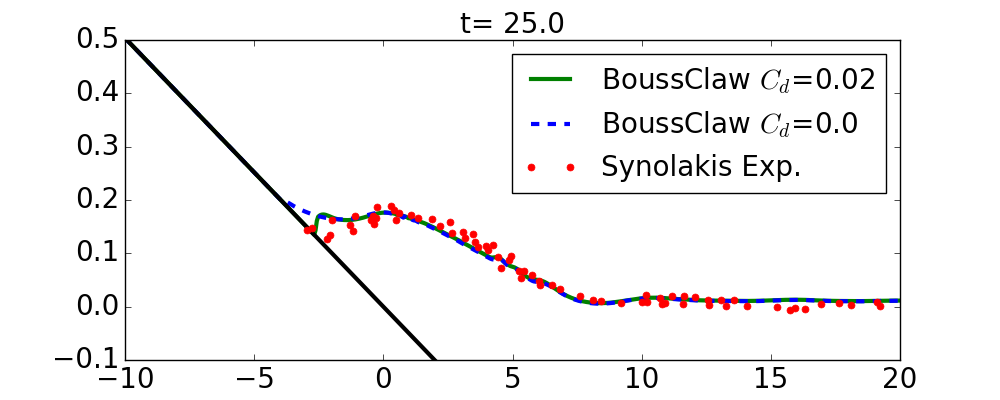
\includegraphics[width=.45\textwidth]{_fig/BoussClaw_lab_Cd_t25}
	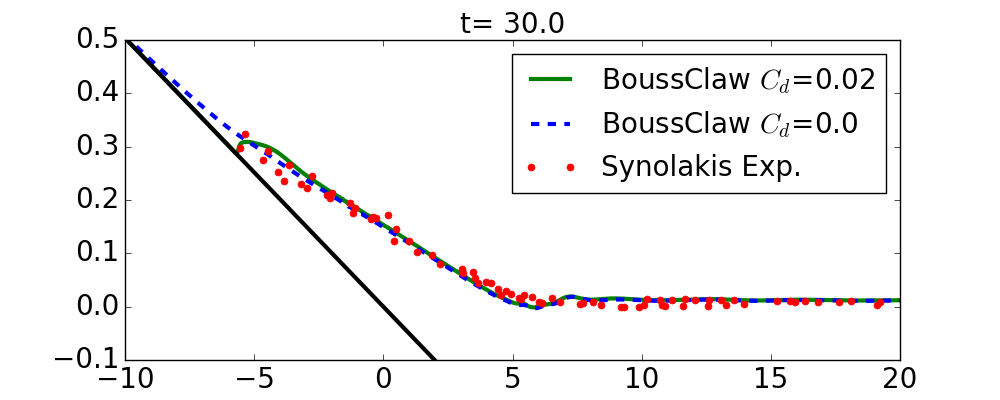
\includegraphics[width=.45\textwidth]{_fig/BoussClaw_lab_Cd_t30}
	\caption{Comparison of experiments and BoussClaw results 
		at t=25 and 30.}
	\label{fig:BoussClaw_runup}
\end{figure}



%The computation of BIM can not proceed further after $t=19.2$ because of the singularity.

%One of the main reasons is to exclude the effect of the bottom friction. Without appropriate inclusion of the friction forces, the numerical results will not yield comparable results with the experiments. When different numerical models are compared, however, it is difficult to distinguish the friction errors from the modeling errors. Therefore, the numerical solution of BIM without any friction is considered as a solution.

%Figure \ref{fig:sw_timeseries} and \ref{fig:bous_timeseries} show the computational results from depth-averaged models, and both models do not capture the wave breaking properly.
%In Figure \ref{fig:bous_timeseries}, the numerical results from the \BoussClaw are given, the amplitude of the incoming wave continues to increase and the wave does not break. 

%\begin{figure}[!htb]
%\centering
%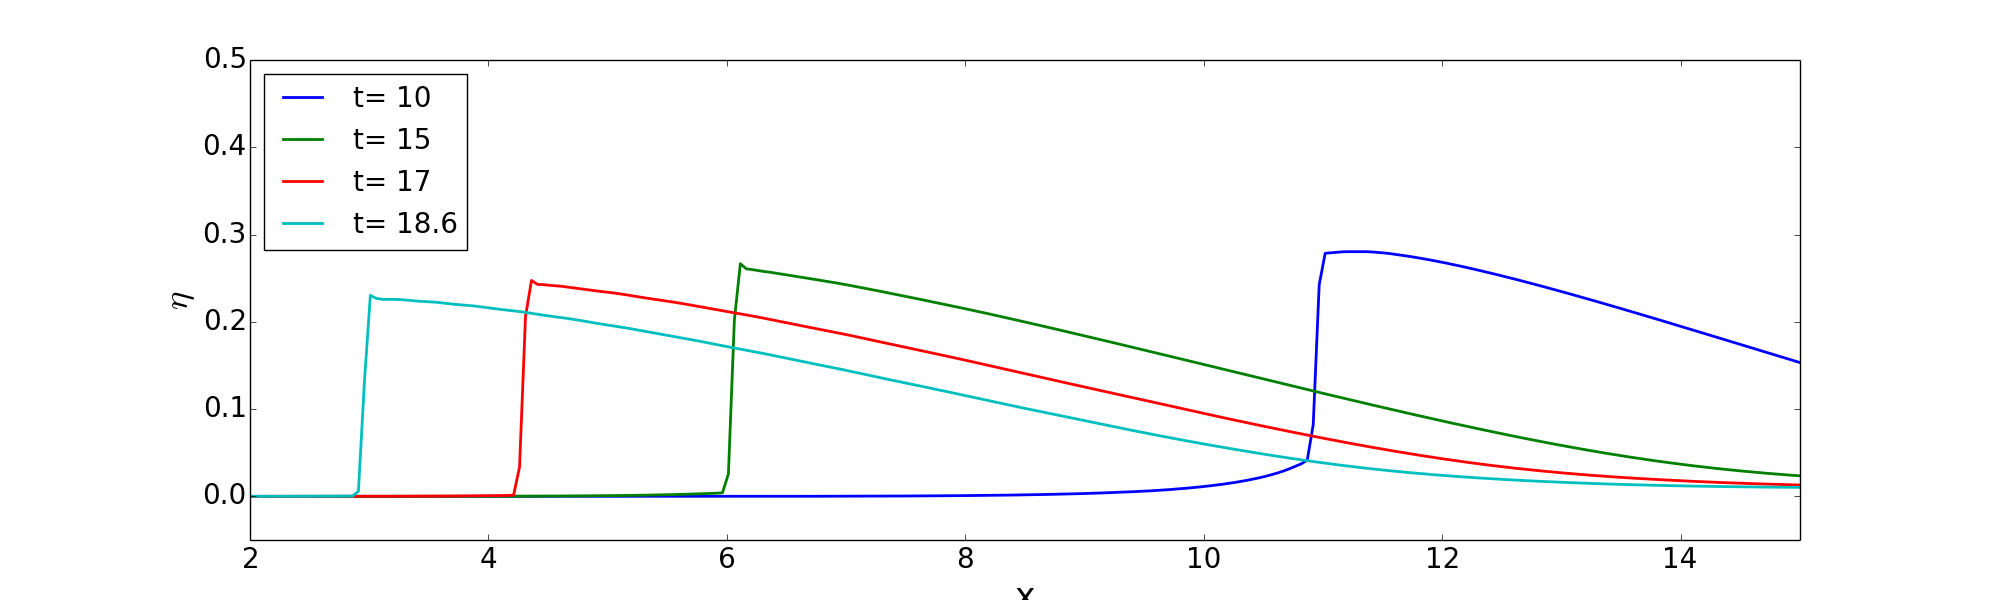
\includegraphics[width=\textwidth]{_fig/sw_dx05_time_series.png}
%\caption{Computational results from NLSW at $t=10,15,17$ and $18.6$.}
%\label{fig:sw_timeseries}
%\end{figure}

%\begin{figure}[!htb]
%\centering
%\includegraphics[width=\textwidth]{_fig/bous_dx025_time_series.png}
%\caption{Computational results from \BoussClaw 
%at $t= 5,9,13,17$ and $20$ s.  }
%\label{fig:bous_timeseries}
%\end{figure}

\section{Shoaling and breaking phenomena}
\subsection{Pre-breaking}
\label{sec:num_breaking}
\citet{wei1995fully} made computation of pre-breaking solitary wave shoaling with
 their fully nonlinear extension of Nwogu's model with full potential 
theory and the weakly nonlinear version of Nwogu's model.
They found that the fully nonlinear Boussinesq equations were superior to those of Nwogu in the later stages of the shoaling.
In this subsection we will do a similar comparison for our models on the $1:19.85$ slope which was not included in the reference.
 
We use the set-up described in section \ref{sec:wave_break} for the Boussinesq modeling of solitary waves on a slope. 
%Figure \ref{fig:bim_boussclaw} shows the snapshots of 
%the water surface at t=$16$ and $18.6$
%from BIM and \BoussClaw with B=$0$ and $1/15$.
%When the wave is smooth at t=16, the \BoussClaw
%results are similar.
%At the breaking point, $t=18.6$, larger differences are observed. 
%If $B=0$, the wave speed is slightly faster 
%than the BIM result, but the wave amplitude is similar. 
%When $B=1/15$, the wave speed matches the BIM results better,
%but the amplitude is slightly smaller. 
%In general, the computational results are rather similar
%with $B=0$ and $1/15$. 
%\begin{figure}[!htb]
%\centering
%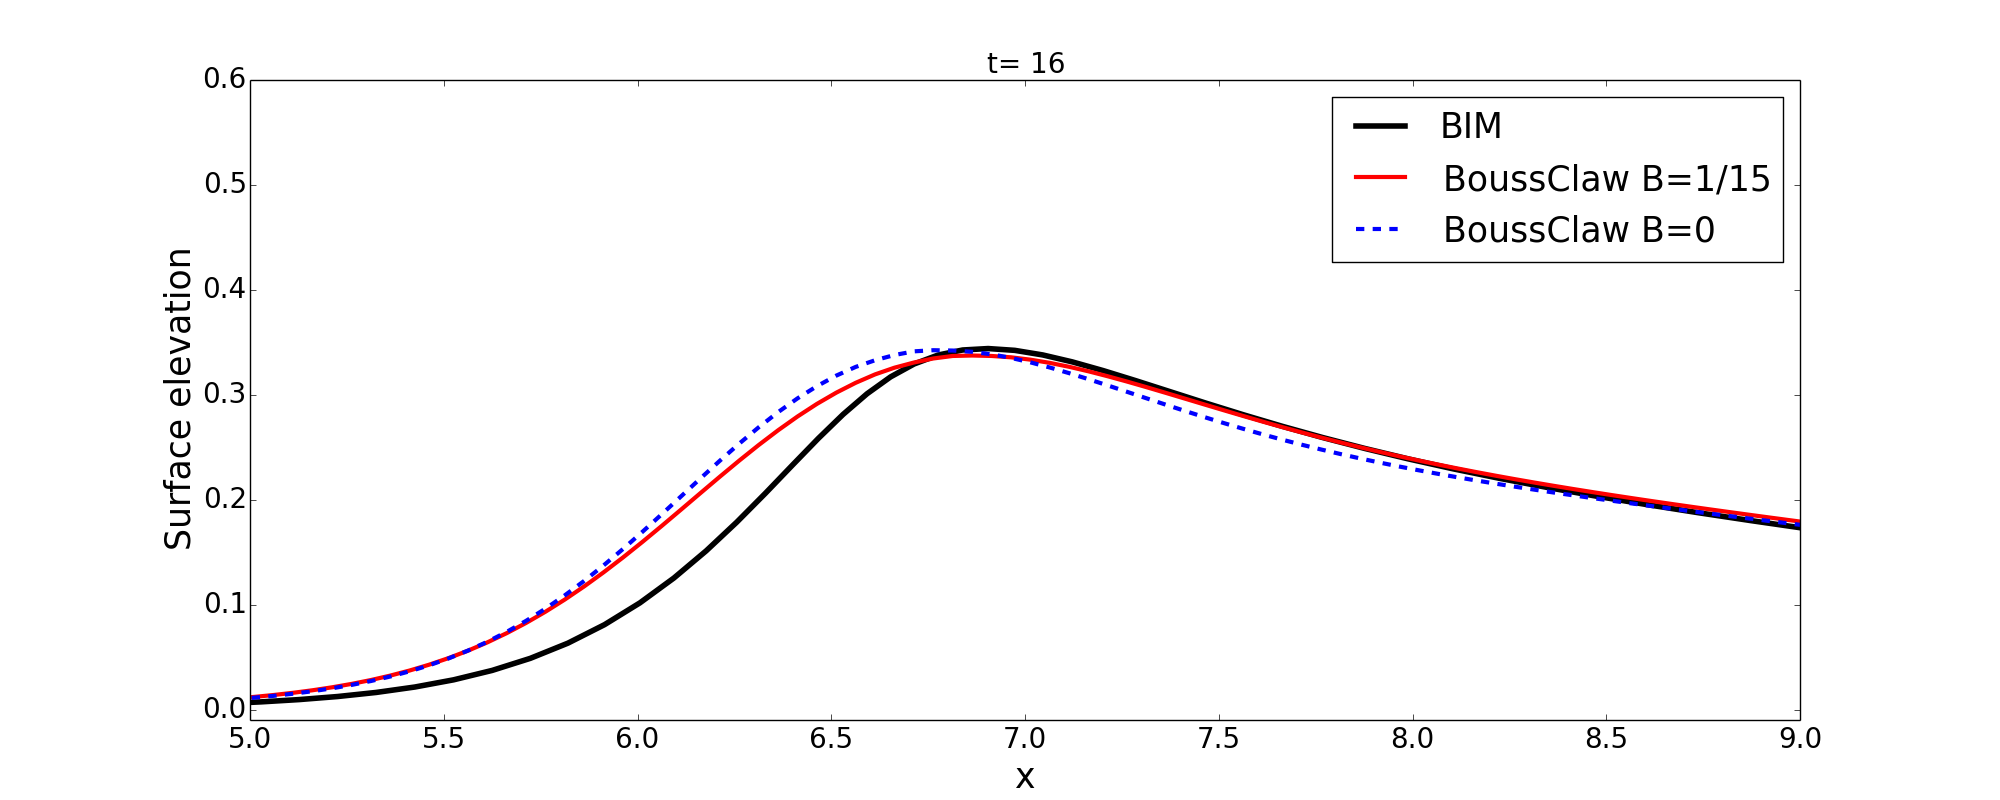
\includegraphics[width=.9\textwidth]{_fig/bim_boussclaw_160.png}\\
%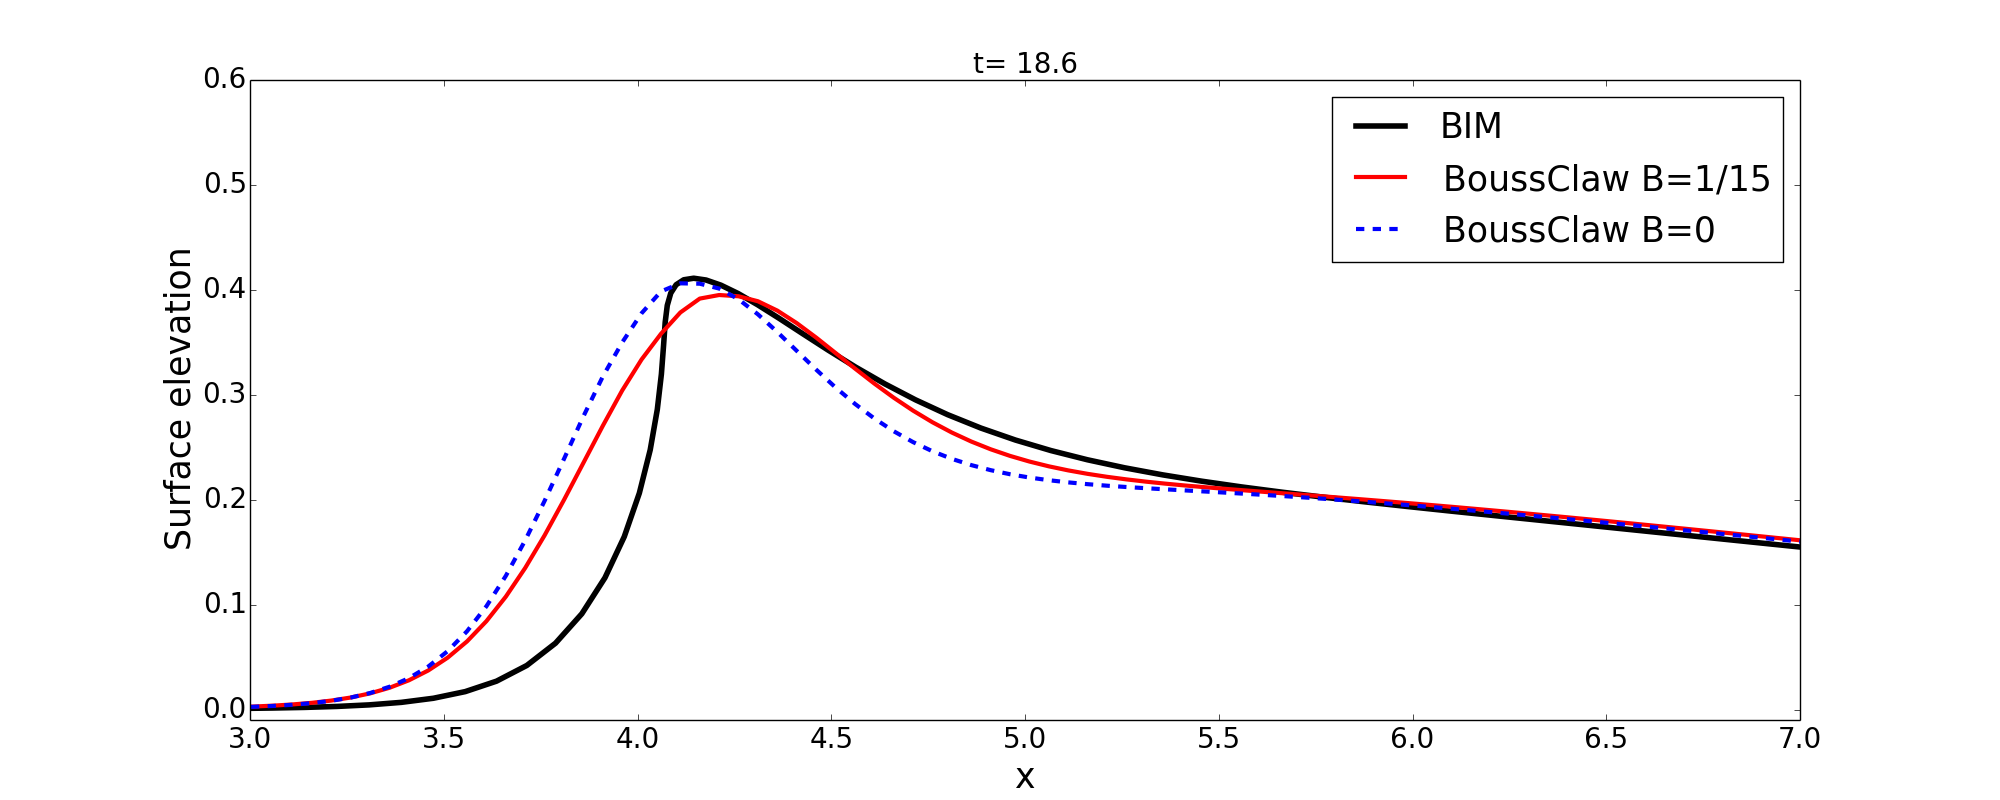
\includegraphics[width=.9\textwidth]{_fig/bim_boussclaw_186.png}
%\includegraphics[width=.7\textwidth]{_fig/bim_boussclaw_192.png}
%\caption{Snapshots of BIM and \BoussClaw with B=$0$ and $1/15$ at t=$16$, and $18.6$.}
%\label{fig:bim_boussclaw}
%\end{figure}
%\marginpar{\footnotesize Lines in figure 10 indistinguishable Change line style or color} 
The \BoussClaw simulations are compared
with those of other Boussinesq solvers, namely
 \textsc{Funwave} \citep{shi2012high}, \textsc{GloBouss} \citep{lovholt2010coupling} and the Serre type formulation \citep{Lovholt:2013a}.
As noted above, 
the original Serre's equations are enhanced by adding the \citet{schaffer1993boussinesq} terms. 
%And the boundary integral method (BIM) for the full potential theory is also considered. 
%The threshold of the wave breaking is not used in this section. 

\begin{figure}[!htb]
\centering
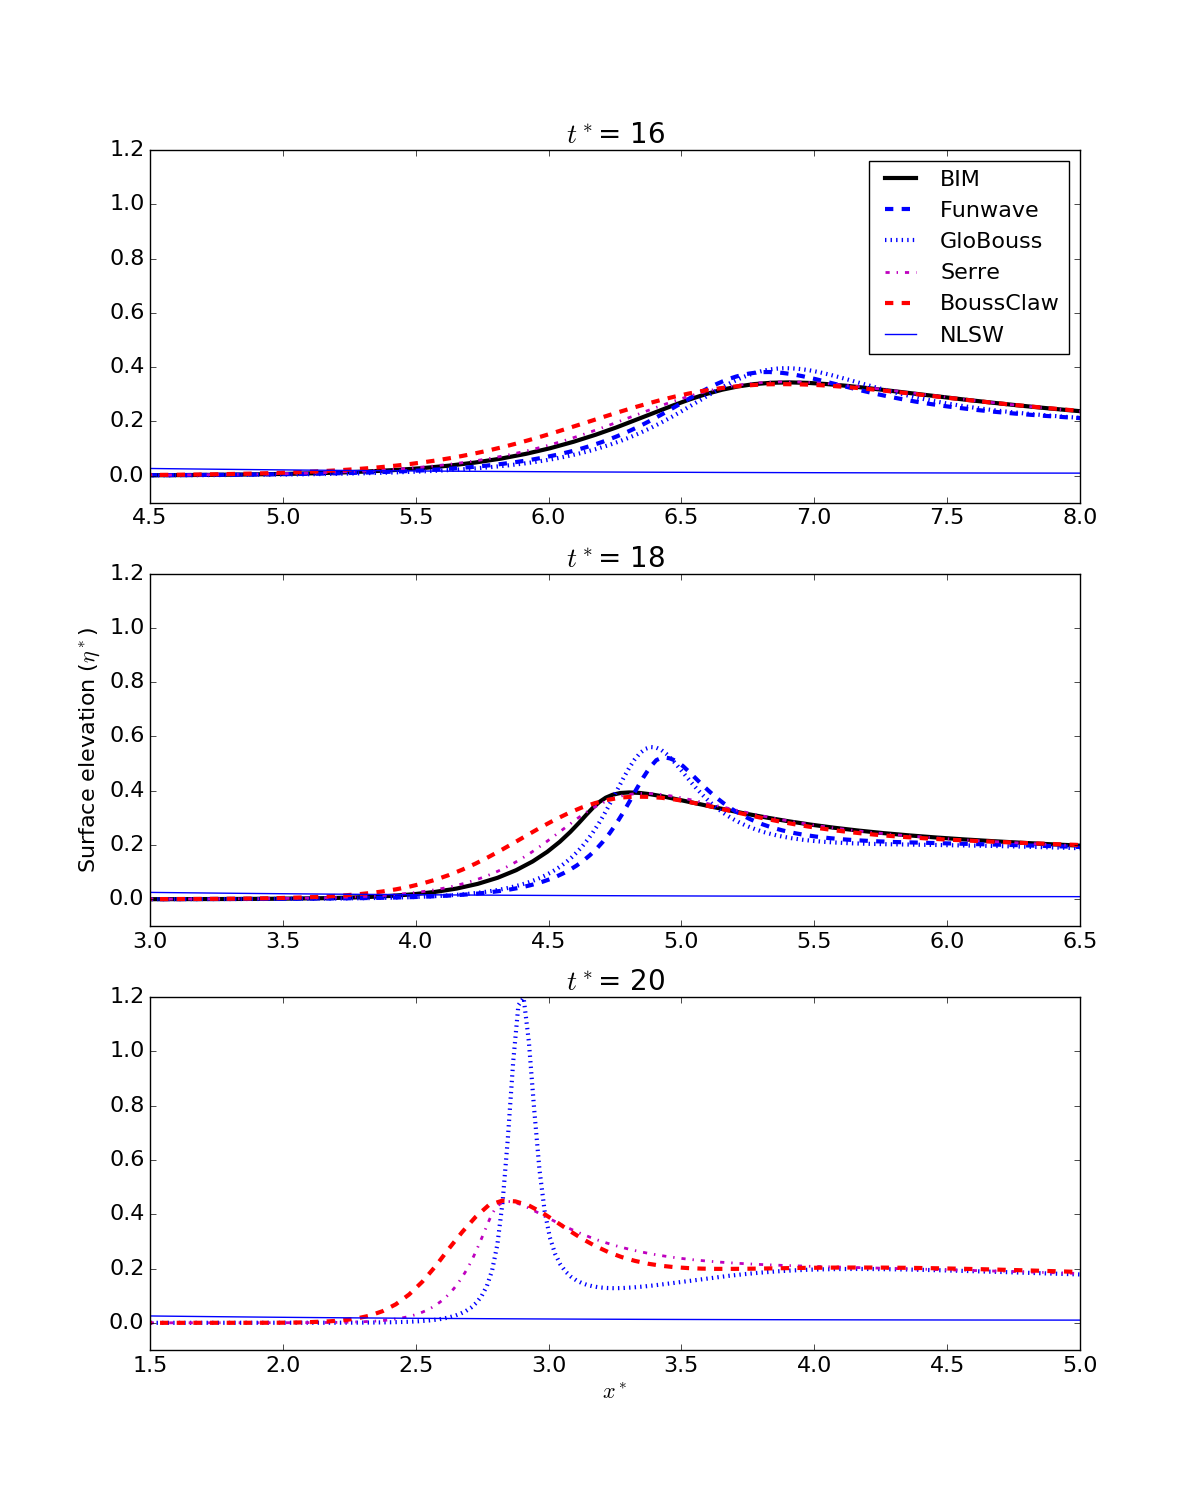
\includegraphics[width=.8\textwidth]{_fig/bim_boussclaw_fun_glob.png}
\caption{Snapshots of BIM, Serre, \textsc{GloBouss}, \BoussClaw
and \textsc{Funwave} at t = $16$, $18$ and $20$.
The \BoussClaw is used with B=$1/15$,
and the Peregrine's form is used for \textsc{GloBouss}.}
\label{fig:bim_boussclaw_fun}
\end{figure}

In Figure \ref{fig:bim_boussclaw_fun}, snapshots from different
numerical models are shown at $t=16$, $18$ and $20$.
At the $t=20$ there are no results from the BIM model as  the wave has broken.
\todo{RJL: Why no BIM solution at t = 20? G: could we include t=19.1 instead, with the BIM in place ?}
For the \BoussClawt, the parameter $B=1/15$ is used, 
but the computational results are rather similar with $B=0$
for this case. 
At t=$16$, the computational results
from all the Boussinesq-type equations show similar results.
The NLSW model, on the other hand, has yieldes a premature breaking 
causing a too low amplitude. Moreover, the wave celerity is also over-estimated
by the hydrostatic model. 
At t=$18$, some discrepancies are observed 
that can be split into two groups, and
\textsc{GloBouss} and \textsc{Funwave} 
are similar while the \BoussClaw
and the Serre results are similar. 
The wave amplitudes computed by the \textsc{GloBouss} and \textsc{Funwave} models,
are more than 20 \% \todo{Is the figure 20\% OK. The old 10 was far too small} larger than those from the BIM model.
The wave amplitude continues to increase 
with \textsc{GloBouss} simulations,
and the difference from the \BoussClaw result 
becomes larger at t = $20$. 
The results from the Serre and \BoussClaw models clearly
more similar to those of the BIM model. 
Especially, the wave amplitudes are correctly determined by these models.
Our observations are in line with those of \citet{wei1995fully}.
 
\subsection{Wave breaking and run-up}
In the BIM model we may identify the onset of breaking according when and where we first observe a vertical slope at the wave front.
For an incident amplitude of $A/h=0.28$ on a $1:19.85$ slope
breaking then starts at $t=18.6$ and $x=4.09$ with $A/h=2.01$.
%\todo{What are the height, time, etc for the BIM simulation}
When the crest in the \BoussClaw simulation reaches $x=4.09$, 
we find
$A/h=1.97$, the ratio of wave speed to celerity ($u/\sqrt{gH}$)
is $1.034$ and maximum surface slope angle of $39.1^\circ$.

For an incident amplitude of $A/h=0.28$ and a $1:19.85$ slope the \BoussClaw model,
the treshold $\epsilon_B=0.8$ (see sec.~\ref{sec_add_num}) is  reached at $t=14.9$
when the peak of the wave is at $x=8.03227$.
In the following, we explore the wave evolution with and without
the application of this threshold.
%At this time, the wave breaking is assumed to start, 
%and the governing equations are switched 
%to the shallow water equations.
%Meanwhile, the BIM results show $x=4.02$ m and  $\epsilon_B=2.01$ at the start of the wave breaking.

\todo{Are there Synolakis data for t=20 ?}
In Figure \ref{fig:boussclaw_th08}, snapshots are shown at 
t=$20$, $25$, and $30$ of the solutions from \BoussClaw and NLSW
with the Manning coefficient $C_d=0.02$.
We compared the NLSW and \BoussClaw with $\epsilon_B=0.8$
and without the threshold. 
At $t=20$ the simulation with $\epsilon_B=0.8$ has already been in NLSW mode for $5$ time units and the difference in the wave height 
from the full Boussinesq simulation is significant. In fact, the treshold solution is closer to the NLSW solution.
is clearly observed. 

At $t=25$ and $t=30$, the wave is running up the slope, 
and the difference in the swash tongue is relatively small. 
On the other hand, while \BoussClaw simulation with $\epsilon_B=0.8$ is
smooth at $t=20$ irregularities are observed
around $x=8$ due to the accumulated errors generated by the splicing of 
Boussinesq and NLSW equations.\todo{How does this eveolve? Is it seen in other paper ?} 

\begin{figure}[tbh!]
\centering
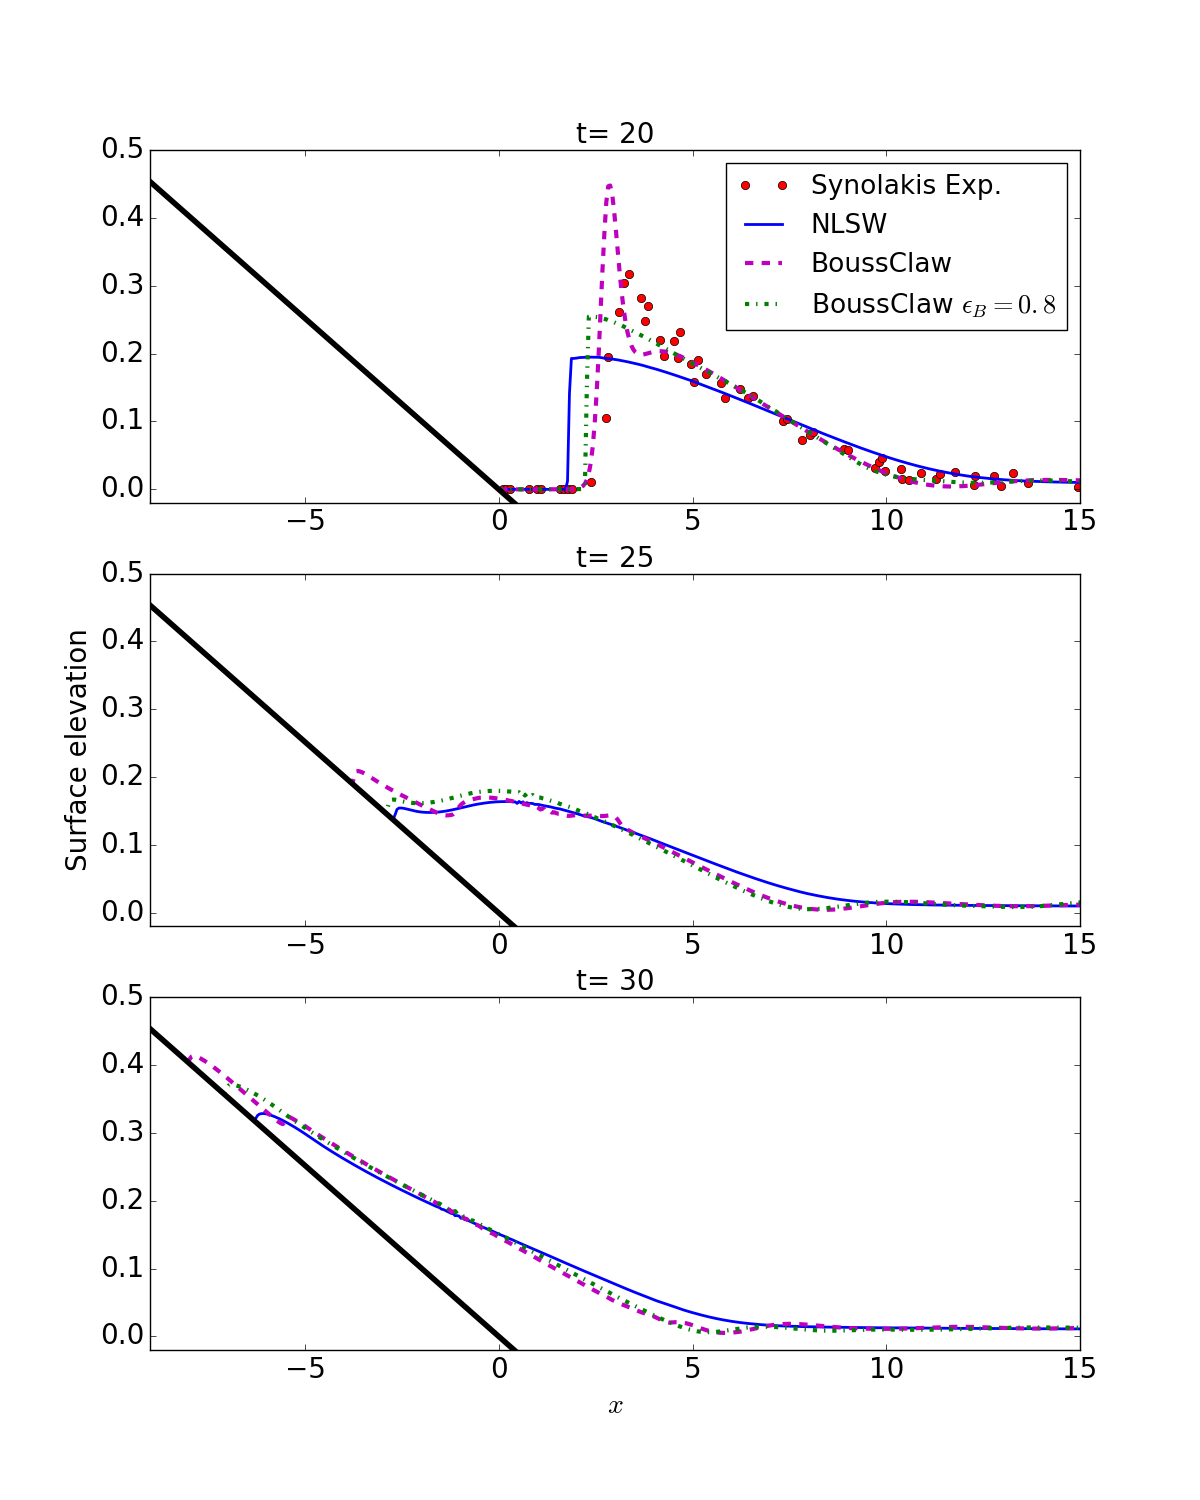
\includegraphics[width=.8\textwidth]{_fig/bim_boussclaw_etaB8}
\caption{Comparison of \BoussClaw and NLSW 
with $\epsilon_B=0.8$ at t =$20$, $25$ and $30$.
Fiction forces have been added with $C_d=0.02$.}
\label{fig:boussclaw_th08}
\end{figure}

Figure \ref{fig:wave_break_criteria} shows 
the amplitude to depth ratio, $\epsilon_B$, as function of the crest location. 

\begin{figure}[tbh!]
\centering
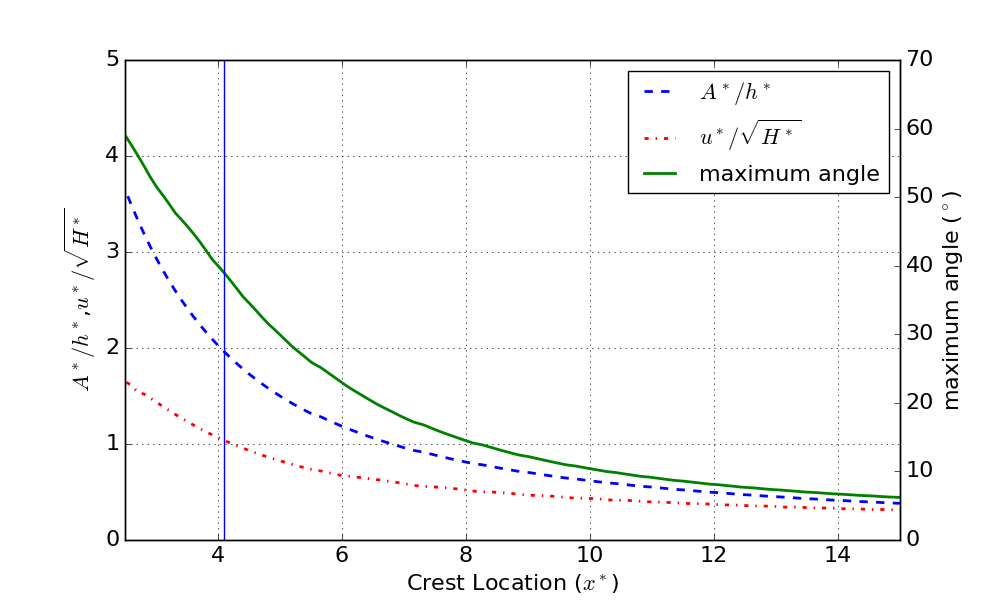
\includegraphics[width=.7\textwidth]{_fig/wave_break}
\caption{Plot of $A/\eta$, $u_s/c$ and maximum angle of waves vs. crest location. 
BIM shows the wave break at $x=4.09$. }
\label{fig:wave_break_criteria}
\end{figure}

\subsection{Wave Energy}

The integrated wave energies  
for the shallow water equations and Boussinesq equations
are $E_0$ and $E_0+E_1$  respectively, 
which are given in (\ref{eq:energy_e0}) and (\ref{eq:energy_e1}). 

\begin{figure}[tbh!]
    \centering
    \begin{subfigure}[b]{0.45\textwidth}
        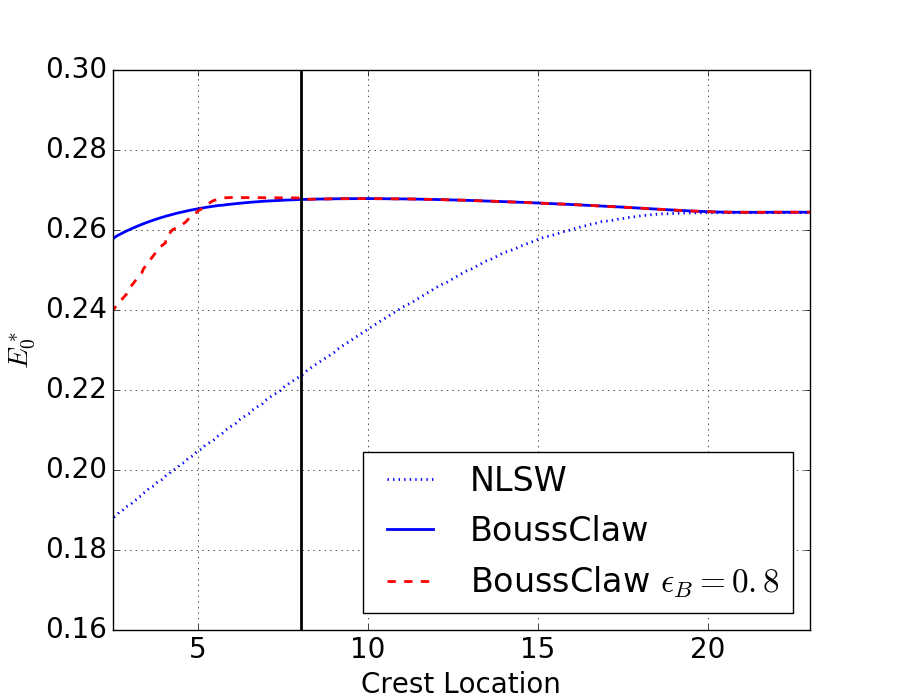
\includegraphics[width=\textwidth]{_fig/e0_boussclaw_eb08.png}
        \caption{$E_0$}
        \label{fig:e0_boussclaw_eb08}
    \end{subfigure}
    \begin{subfigure}[b]{0.45\textwidth}
        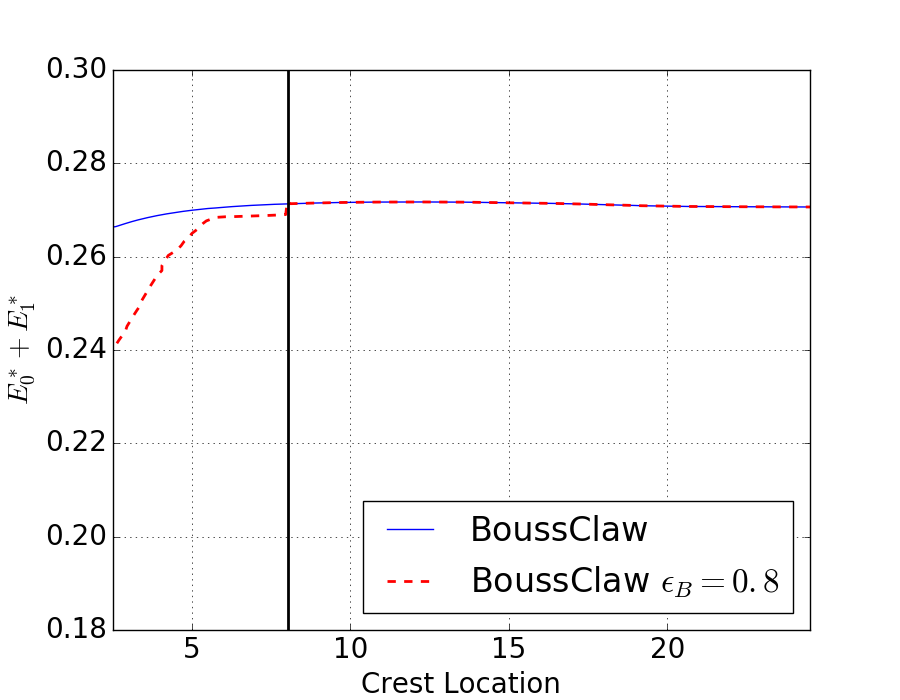
\includegraphics[width=\textwidth]{_fig/e1_boussclaw_eb08.png}
        \caption{$E_0+E_1$}
        \label{fig:e1_boussclaw_eb08}
    \end{subfigure}
    \caption{Energy plots of NLSW and \BoussClaw.
    The vertical line is at $x=8.03227$ m where $\epsilon_B=0.8$,
    and the governing equations are switched to the NLSW from
    the Boussinesq equations. }
    \label{fig:energy_boussclaw_swe}
\end{figure}

In Figure \ref{fig:energy_boussclaw_swe} the energy densities are depicted as 
functions of the crest location, $x_c$. 
In the left panel 
we observe that the $E_0$ is nearly constant 
for the shallow water equations until a shock is formed around $x_c=13$.
Thereafter, energy is quickly dissipated. 
In  the \BoussClaw simulation with no treshold (right panel) 
$E_0+E_1$ is nearly when the wave propagates in constant depth. 
On the deeper parts of the slope there is first a very moderate increase, then a
very gentle reduction. This may be due to the absence of strict energy  conservation in the Boussinesq equations in the first place. 
Close to the shoreline there is stronger, but still mild, energy dissipation.
When the threshold $\epsilon_B=0.8$ is invoked there is no difference from the full Boussinesq solution until the the treshold is reached for 
 $x_c=x_B=8.03227$. Then, in fact, there is marked increase in $E_0+E_1$ followed by a stronger  reduction then for the full solution.
The increase is presumeably a consequence of errors introduced by changing the 
governing equations from a Boussinesq to a NLSW type. 
After  $x_c=x_B$  
the hydrostatic energy measure, $E_0$, may be appropriate in this case.
The artificial energy maximum  is then reduced and is only slightly higher than
the general overshoot for $E_0$ and Boussinesq equations for $x_c>x_B$.  
\todo{G: Most appropriatly $e_0$ should be integrated from the NLSW part, while $e_0+e_1$ should be used elsewhere. How to conclude ?  }

\section{Conclusion}
\label{sec:conclusion}

In the present paper we have presented a new  
Boussinesq type model, \BoussClawt,
for modeling fully non-linear dispersive tsunami propagation, taking also into account drying-wetting during inundation and withdrawal on the beach.
\BoussClaw resembles much used general purpose models such as \textsc{Funwave-TVD} and
\textsc{Coulwave-TVD}, but is based on a slightly simpler and more transparent set of governing equations,
and has a slightly different numerical scheme. We have tested numerical implementation towards
analytical solitary wave expressions as well as laboratory experiments.

Making use of the experiments of \citet{synolakis1987runup} 
enabled us to
constrain a set of different long wave models, including \BoussClawt, as well as a full potential
BIM reference model. Using the BIM, we were able to explore in detail the post-breaking behaviour,
and to identify the point of breaking accurately. This was useful for determining the 
validity of the respective long wave models. First, we found that by using standard NLSW models,
the point of breaking will be located too far offshore. Boussinesq models
provide the opportunity of providing a more accurate description of the near shore propagation and shoaling. 
However, in current practise the Boussinesq terms are often omitted near shore through the $A/h>0.8$ threshold criteria.
As a consequence, the point of breaking may be misinterpreted also in Boussinesq type models.

In the present example, we investigated the near shore propagation over a relatively gentle shelf of $1/19.85$ slope,
and in this case the actual onset of breaking occurred for $A/h \approx 2$, which is significantly later
than what would be predicted in any standard approach (NLSW or Boussinesq). As demonstrated in this paper,
the combined effects of non-linearities and dispersion influence the solution markedly, when accumulated to the point
of breaking. It is noted that the artificial effect discovered would depend on the slope, 
and the $A/h=0.8$ limited may well work better on a much gentler slope as it is primarly derived based on 
solitary wave evolution on constant depth. On the other hand, $1/19.85$ slope is already quite gentle,
and the offset between the reference solution and Boussinesq models using this criteria may
be even more pronounced for steeper slopes.

%{\em What should the main conclusions be}
%\begin{itemize}
%\item \BoussClaw works.
%\item Shallow water models and composite Boussinesq/NLSW models
%      may give large errors in breaking point and wave shape
%\item Breaking does not really occur before the local amplitude is much higher than 0.8 time the depth -- a limit that is inspired by the existence of solitary wave solution in full potential theory.
%The 0.8 limit  may be better on even gentler slopes.
%\item Effects of nonlinearities in the dispersion does influence the solution markedly, when accumulated up to the point of breaking.
%\end{itemize}

\section*{Temporary section: What to do}
These are in addition to margin-notes.
\begin{enumerate}
\item Add references to introduction.
\item More figures for section \ref{sec:10degrunup}; snapshots, shorelines 
maximum runup, convergence.
\item Grid increments must be described, somehow, for all results.
\item What to say about breaking performance ?
\item Old figures 9b, 10bc. Reinserted ?
\end{enumerate}

\appendix

\section{Stability of the hybrid scheme}
\label{append:stab}
It is difficult to analyze the numerical stability for  our full Boussinesq
equations. 
To obtain some insight in the  stability of the proposed hybrid numerical scheme,
we thus consider a closely related, but simpler, equation, namely the 
linearized Benjamin-Bona-Mahony (BBM)
equation (\cite{benjamin1972model}) 
\begin{align}
u_t + c u_x = \frac{h^2}{6}u_{txx},
\label{eq:basic_1}
\end{align}
where $c=\sqrt{gh}$.
This equation describes weakly dispersive, uni-directional waves in constant
depth. The equation replaces the momentum equation, whereas no separate
continuity equation is involved.

Following the steps of section \ref{sec:Num_scheme},
we rearrange 
the equation (\ref{eq:basic_1}) as
\begin{align}
(I-D)(u_t + c u_x) +Du_x = 0, \label{eq:basic_2}
\end{align}
where $D=\frac{h^2}{6}\partial_x^2$.
The first step of  hybrid scheme for  this equation is integration of
 the advection equation
\begin{align}
u_t + c u_x = 0,
\label{eq:append_advec}
\end{align}
by the finite volume method. 
Then the Runge-Kutta  method is applied to,
\begin{align}
(1-D)u_t + cDu_x = 0.
\label{eq:append_mom_fdm}
\end{align}
which is the counterpart to  (\ref{eq:hybrid_mom_fdm}).

If we use the centered spatial difference approximation of $O(\Delta x^2)$
accuracy on a regular grid we may employ a standard von Neumann analysis where we calculate the growth of an harmonic mode over a single time step.
Expressing the coefficients of the velocity array before the time step as  $u_j= e^{i\xi j \Delta x}$ we then replace the coefficient of $\textbf{M}^q$, defined in section \ref{sec:Num_scheme}, 
by $M_j^q=U_j^q= g^qe^{i\xi j \Delta x}$, 
where $q$ is 1, 2, 3, 4 or +. Correspondingly, the coefficients of the $\mathbf{S}^k$ array, which contains auxiliary,  nodal values for $u_t$,  is
expressed $(S_j^k)= s^k e^{i\xi j \Delta x}$. 

The stability  of the first step, (\ref{eq:append_advec}),  is assured by the standard CFL criterion
\[\frac{c\Delta t}{\Delta x} <1.\]
If we instead solve the NLSW equations, as in \BoussClawt, $c$ must be replaced by the nonlinear characteristic velocity, which may lead to a more strict criterion. However, the method employed in the first step is not suited for a von Neumann stability analysis and we thus apply this technique to the second step only. 
 Hence, we may put $g^1$ to unity, but it is preferable to retain it in the calculations. 
The Runge-Kutta scheme for time stepping, (\ref{eq:rk4_S}), may  now be
expressed as
\begin{flalign} 
g^2 = g^1 + \frac{\Delta t}{2}s^1, \quad
g^3 = g^1 + \frac{\Delta t}{2}s^2, \quad
g^4 = g^1 + \Delta t s^3,
\label{eq:rk4_Neumann}
\end{flalign}
The discrete version of (\ref{eq:append_mom_fdm}), which is the counterpart to
(\ref{eq:rk4_1}) for the BBM equation reads 
\begin{align*}
& S_j^k - \frac{h^2}{6}\frac{S_{j+1}^k-2S_j^k+S_{j-1}^k}{\Delta x^2} = 
-\frac{ch^2}{6}\frac{U_{j+2}^k - 2U_{j+1}^k +2U_{j-1}^k -U_{j-2}^k}{2\Delta x^3},
\end{align*}
which, inserted the harmonic expressions, implies
\begin{align}
s^k=i \frac{\gamma}{\Delta t} g^k,\quad \gamma = c\Delta t \frac{ 2\sin(\xi \Delta x)(1-  \cos(\xi \Delta x)) }
                     { 6\Delta x^3h^{-2} +2\Delta x(1-\cos(\xi \Delta x))},
\label{append:rk4_1}
\end{align}
where the $\Delta t$ factors are included for convenience.
The assembling of the intermediate values in the Runge-Kutta procedure, 
(\ref{eq:rk4_assemble}), now yields 
\begin{flalign}
g^+ & = g^1 + \frac{\Delta t}{6} \left[
s^1+2s^2+2s^3+s^4
\right]. 
\label{append:rk4_assemble}
\end{flalign}

By combination of (\ref{eq:rk4_Neumann}) and (\ref{append:rk4_1}) $s^k$ and $g^k$, $k=1..4$ can be calculated successively  and combined in (\ref{append:rk4_assemble}) to provide
the value of $g^+$, 
\begin{align*}
g^+(\gamma) & = \left(1-
\frac{1}{2}\gamma^2 +\frac{\gamma^4}{24} + \left(\frac{\gamma^3}{6} -\gamma \right)i\right)g^1 \\
|g^+(\gamma)|^2 & = \left(1 + \frac{1}{4}\gamma^4 + \frac{\gamma^8}{24^2} -\gamma^2 + \frac{\gamma^4}{12}
-\frac{\gamma^6}{24} + \gamma^2 + \frac{\gamma^6}{36} -\frac{\gamma^4}{3}\right)|g^1|^2 \\
& = \left(1 -\frac{1}{72}\gamma^6 + \frac{1}{576}\gamma^8\right)|g^1|^2.
\end{align*}
Stability requires  $|g^+(\gamma)/g^1|<1$ which is 
equivalent to  $|\gamma|<2\sqrt{2}$. Moreover, it is easily seen that 
$\gamma<c\Delta t/\Delta x$. 
Hence, a sufficient condition for stability of the second step of the hybrid scheme is 
\[
\frac{c\Delta t}{\Delta x} < 2\sqrt{2}.
\] 
This is more relaxed than the CFL condition for the advection equation
(\ref{eq:append_advec}). 
Therefore, if the CFL condition is satisfied in the advection equation,
the fractional step is always stable with the suggested numerical scheme. 


\section{Energy estimates and dissipation}
\label{append:energy}

\subsection{Velocity field}

To derive the energy estimates for the Boussinesq-type equations, 
we define the depth-averaged velocity as,  
\begin{flalign*}
\bar{u} = \frac{1}{H}\int_{-h}^{\epsilon \eta} u dz .
\end{flalign*}
Then the velocity $u$ can be expressed as
$u = \bar{u} + \mu^2 u_1$ where
\begin{align}
\int_{-h}^{\epsilon \eta} u_1 dz=0. \label{eq:avg_u1}
\end{align}
Then the kinematic boundary condition at the bottom and zero divergence
implies
\begin{flalign*}
w = -h_x u  - \bar{u}_x (z+h) + O(\mu^2). 
\end{flalign*}

\subsection{Energy integrals}

The potential energy density per horizontal area is 
\begin{flalign*}
V = \int_{-h}^{\epsilon \eta} g z dz = \frac{1}{2}\epsilon^2 g \eta^2 
- \frac{1}{2} g h^2, 
\end{flalign*}
where the last term $\frac{1}{2} g h^2$ is the equilibrium energy.
The kinematic energy density has two contributions,
\begin{flalign*}
T=T_u+T_w; 
\quad T_u = \frac{1}{2}\epsilon^2 \int_{-h}^{\epsilon \eta} u^2 dz, 
\quad T_w = \frac{1}{2}\epsilon^2 \mu^2 \int_{-h}^{\epsilon \eta} w^2 dz. 
\end{flalign*}
For the horizontal part, $T_u$ is 
\begin{flalign*}
T_u = \frac{1}{2}\epsilon^2 \int_{-h}^{\epsilon \eta} u^2 dz
= \frac{1}{2}\epsilon^2 \int_{-h}^{\epsilon \eta} 
\bar{u}^2+2\mu^2\bar{u}u_2 + \mu^4u_1^2 dz
= \frac{1}{2}\epsilon^2 H \bar{u}^2 + O(\epsilon^2 \mu^4),
\end{flalign*}
since $\bar{u}$ is independent of $z$ and by (\ref{eq:avg_u1}).
Assuming $\frac{1}{H}\int_{-h}^{\epsilon \eta} u^2 dz = \bar{u}^2$,
the vertical part is 
\begin{flalign*}
\quad T_u & = \frac{1}{2}\epsilon^2 \mu^2 \int_{-h}^{\epsilon \eta} 
h_x^2u^2 +2h_xu\bar{u}_x(z+h)
+ \bar{u}_x^2 (z+h)^2 dz + O(\epsilon^2\mu^4) \\
& = \frac{1}{2}\epsilon^2 \mu^2 H
\left(
h_x^2 \bar{u}^2 + H h_x\bar{u} \bar{u}_x + \frac{1}{3} H^2 \bar{u}_x^2
\right) + O(\epsilon^2\mu^4).
\end{flalign*}
Thus the energy of a wave can be approximated as 
\begin{flalign*}
& e = \epsilon^2 \left( e_0 +\mu^2 e_1 + O (\mu^4)\right)
\end{flalign*}
where
\begin{flalign*}
& e_0 = \frac{1}{2}\left( g\eta^2 + H\bar{u}^2 \right), \\
& e_1 = \frac{1}{6}H^3\bar{u}_x^2
+ \frac{1}{2}H^2h_x\bar{u}\bar{u}_x + \frac{1}{2}Hh_x^2\bar{u}^2.
\end{flalign*}

\section*{References}

\bibliography{mybibfile}

\end{document}
\grid
